%This document contains Liza's update (as of December 2016) of abstract, intro, part 1, and appendix 1 
\documentclass[12pt,twoside,a4paper,notitlepage]{article}
%\documentclass[preprint,authoryear]{article} 
\usepackage{indentfirst}
\usepackage [english]{babel}
%\usepackage[utf8]{inputenc}
%\usepackage{times} %this package has impact on fonts of output
\usepackage[utf8]{inputenc} %this package allows reading French accented letters directly
\usepackage[T1]{fontenc} %this package makes hyphenated characters such as umlauts available in latex
\usepackage{amsmath} 
\usepackage{amssymb} %ams symbols (\mathbb fonts}
\usepackage{amscd} %draws commutative diagrams
\usepackage{bm} %bold mat fonts(\mathbm)
\usepackage{graphicx,pst-all} 
%\usepackage{graphicx}
\usepackage{hyphenat} %enables control over hyphenation 
\usepackage{fancyvrb,moreverb} %verbatim
\usepackage{float} %enables float [H] option: useful for putting figures in the text
\usepackage{mathptmx}
\usepackage{amsthm}
\usepackage{newtxtext,newtxmath}
\usepackage{mathrsfs} %more math symbols (viz., \mathscr)
\usepackage{textcomp} %this package helps with writing symbols
\usepackage[gen]{eurosym}
\usepackage{epstopdf}
\usepackage[strict]{changepage}
\usepackage{enumerate}
\usepackage[margin=2.5cm]{geometry}
%\usepackage[letterpaper]{geometry}
%\geometry{verbose,tmargin=1cm,bmargin=1cm,lmargin=0.95cm,rmargin=0.95cm}
%\usepackage[usenames]{color}
\usepackage{color}
\usepackage{verbatim}
%\usepackage{setspace}
%\doublespacing
%\linespread{1.6} %this gives double spacing throughout the document
\linespread{1.3}
%this package sets the spacing preferences
\usepackage{natbib}
%\usepackage[authoryear]{natbib}
\usepackage[unicode=true, pdfusetitle, bookmarks=true,bookmarksnumbered=false,bookmarksopen=false,  breaklinks=true,pdfborder={0 0 0},backref=false,colorlinks=true]{hyperref}
\hypersetup{linkcolor=blue, citecolor=black, urlcolor=black}
%these packages define how links to footnotes and to bibliography items are presented in the paper
%\newcounter{prop}[subsubsection]
%\renewcommand{\theprop}{\roman{prop}}
\usepackage{relsize} %newly added package to use command \mathlarger{}
\usepackage{mathtools} %newly added package to use command \mathrlap{}
\usepackage{tabularx}
\usepackage{booktabs}
\usepackage{caption}
\usepackage{footmisc}


\makeatletter

\usepackage{amsfonts}


\@ifundefined{definecolor}
 {\@ifundefined{definecolor}
 {\@ifundefined{definecolor}
 {\@ifundefined{definecolor}
 {\usepackage{color}}{}
}{}
}{}
}{}

\usepackage{caption}
\usepackage{psfrag}
\usepackage{subfigure}
\usepackage{epsfig}


\usepackage{array}

\usepackage{url}


\urlstyle{same}
\renewcommand{\baselinestretch}{1.5}
\makeatother

%\justifying

%\setlength{\parindent}{20pt} %this command impedes paragraphs' indenting
%\setlength{\parskip}{-4ex plus 0.2ex minus 0.2ex} %this command says how spaces between paragraphs can eventually vary so as to fit on the page

\makeatletter
%\bibliographystyle{plain}
\bibliographystyle{chicago}
%\bibliographystyle{aer}
%\bibliographystyle{phjcp} %alternative biblio styles which look ok
%\bibliographystyle{acm}
%\bibliographystyle{ieeetr}
\bibpunct{(}{)}{;}{d}{,}{,}
\makeatother

\long\def\symbolfootnote[#1]#2{\begingroup%
\def\thefootnote{\fnsymbol{footnote}}\footnote[#1]#2\endgroup}
%\symbolfootnote[1]{footnote} %this line should be used for the footnote to get the symbol between 1-9 but I don't understand how to use it
%\renewcommand{\thesection}{\Roman{section}}
%\renewcommand{\thesubsection}{\thesection.\arabic{subsection}}
%\renewcommand{\thefootnote}{\alph{footnote}} \this changes symbols used for footnotes in body of text

\makeatletter
\newlength{\myFootnoteWidth}
\newlength{\myFootnoteLabel}
\setlength{\myFootnoteLabel}{1.2em}
\renewcommand{\@makefntext}[1]{
  \setlength{\myFootnoteWidth}{\columnwidth}
  \addtolength{\myFootnoteWidth}{-\myFootnoteLabel}
  \noindent\makebox[\myFootnoteLabel][r]{\@makefnmark\ }
  \parbox[t]{\myFootnoteWidth}{#1}
}
\makeatother
\newtheorem{theorem}{Theorem}
\newtheorem{acknowledgement}[theorem]{Acknowledgement}
\newtheorem{algorithm}[theorem]{Algorithm}
\newtheorem{axiom}[theorem]{Axiom}
\newtheorem{case}[theorem]{Case}
\newtheorem{claim}[theorem]{Claim}
\newtheorem{conclusion}[theorem]{Conclusion}
\newtheorem{condition}[theorem]{Condition}
\newtheorem{conjecture}[theorem]{Conjecture}
\newtheorem{corollary}[theorem]{Corollary}
\newtheorem{criterion}[theorem]{Criterion}
\newtheorem{definition}[theorem]{Definition}
\newtheorem{example}[theorem]{Example}
\newtheorem{exercise}[theorem]{Exercise}
\newtheorem{lemma}[theorem]{Lemma}
\newtheorem{notation}[theorem]{Notation}
\newtheorem{problem}[theorem]{Problem}
\newtheorem{proposition}[theorem]{Proposition}
\newtheorem{remark}[theorem]{Remark}
\newtheorem{solution}[theorem]{Solution}
\newtheorem{summary}[theorem]{Summary}
%\newenvironment{proof}[1][Proof]{\textbf{#1.} }{\ \rule{0.5em}{0.5em}}


\newcommand{\noteLA}[1]{\textcolor{blue}{\footnotesize\textit{{noteLA: #1}}}} %this defines a new command for notes which has one argument
\def\noteLA #1{} %when activated, suppresses printing notes - remember to de-activate with %sign when sending draft text
%define another one for Guillaume, for example:
\newcommand{\noteGD}[1]{\textcolor{red}{\footnotesize{noteGD: #1}}} %this defines a note command which has one argument
\def\noteGD #1{} %when activated, suppresses printing notes - remember to de-activate with %sign when sending draft text
\newcommand{\revLA}[1]{\textcolor{red}{\footnotesize\textit{{revLA: #1}}}} %this defines a new command for notes which has one argument
\def\revLA #1{} %when activated, suppresses printing notes - remember to de-activate with %sign when sending draft text


\pagestyle{plain}
\begin{document}
\linespread{1}
\author{Elizaveta Archanskaia\thanks{KU Leuven.}\and Guillaume Daudin\thanks{Université Paris-Dauphine, PSL University, CNRS 8007, IRD 260, LEDa, DIAL, 75016 Paris; SciencesPo, OFCE, 75007 Paris; email: guillaume.daudin@dauphine.psl.eu (Corresponding author)
}}

\title{Product substitutability and the Distance Puzzle\thanks{This paper has greatly benefited from helpful discussions with Thomas Chaney, Anne-C\'elia Disdier, Peter Egger, Lionel Fontagn\'e, Raphaël Franck, Joseph Francois, Guillaume Gaulier, Samuel Kortum, Jacques Le Cacheux, Philippe Martin, Thierry Mayer, and suggestions by seminar participants at the ETSG, the AFSE, the Ljubljana Empirical Trade Conference (Forum for Research in Empirical Internation Trade), the international workshop on the Economics of Global Interactions (Bari), at the Economics Department of SciencesPo, and at the International Trade Working Group at the University of Chicago.
We thank Christian Broda, Natalie Chen, Dennis Novy, and David Weinstein for giving us access to their programs.
The usual disclaimers apply.}}
%previous title: Heterogeneity and the Distance Puzzle
\date{April 2019
\\
}

\maketitle
\begin{abstract}
%95 words
%\linespread{1.3}
We propose a novel explanation of the non-decreasing distance elasticity of trade over 1963-2013, commonly referred to as `the distance puzzle'.
Consistently with previous work, we find that the changing composition of world trade has contributed to making trade less rather than more sensitive to distance.
%reduced the magnitude of the distance puzzle.

Our original contribution consists in documenting a 35\% increase in the perceived substitutability of products traded on the world market over the same period.
We find that the Armington elasticity of substitution increased from about 1.7 to 2.3 between 1963 and 2013.
This elasticity corresponds to the elasticity of trade flows to trade costs on the intensive margin.
In the Armington framework it determines the elasticity of trade flows to trade costs.
The evolution of this parameter suffices to explain the non-decreasing distance elasticity of trade.

\end{abstract}

\textit{Keywords}: gravity equation, distance puzzle, trade elasticity, trade costs

\textit{JEL codes}: F15, N70
\clearpage

\section*{Introduction}
%%We document evolution 1962-2013 while Disdier and Head focussed their meta-analysis on 1870-2001.
%Bosquet and Boulhol (2015) use data in 1948-2006; Berthelon and Freund use data for 1985-2005.
%Head and Mayer (2014) update the Disdier and Head sample to papers published in 2001-2012 while Head and Mayer (2013) investigate the persistence of the distance effect on trade using cross-sectional gravity estimates of the distance coefficients in 1960-2005 (both loglinear and PPML).
%The estimated effect of distance in gravity equations has unambiguously increased over the last 60 years.

It is a well-established fact that trade has not become less sensitive to distance over the last 60 years.
Technological developments in transportation and communication, e.g. the airplane, the container, and the internet were initially expected to lead to the ``death of distance'' by the end of the 20\textsuperscript{th} century.\footnote{\cite{Cairncross1997,Levinson2006,Friedman2007}}
Yet, a larger share of world trade is conducted at short distances now than in the 1960s.
This increase in the distance elasticity of trade, notwithstanding technological developments, has been dubbed the ``distance puzzle''.
More precisely, \cite{Disdier2008} adopt a meta-analytical approach and find that distance impedes trade by 37\% more in the 1990s than it did from 1870 to 1969.\footnote{See also \cite{Berthelon2008,Combes2006, Brun2005, Buch2004}.}
%Berthelon and Freund document a 10\% increase in the distance elasticity over 1985-2005. 
\cite{Head2013} estimate the distance elasticity of trade in successive cross-sections and find that it has doubled in 1960-2005.

%Krautheim(2012) and Chaney(2016)
We investigate the empirical relevance of a mechanism that may help to rationalize the distance puzzle.
We make the simple point that the flattening out of the world may go hand in hand with a persistent impeding effect of distance on trade if consumers perceive product bundles shipped out by each country to the world market as increasingly substitutable.\footnote{Equation (4) in \cite{Head2013}: the distance effect is a product of two elasticities, the elasticity of trade to trade costs and the elasticity of trade costs to distance.
We investigate the evolution of the former.}

\begin{figure}[h!]
	\caption{Dispersion of the number of products exported by each country \label{fig:vioplot}}
	\begin{center}
		\setlength{\fboxrule}{1pt} %makes border lines thick
		\setlength{\fboxsep}{.1in} %increases distance to border
		\fbox{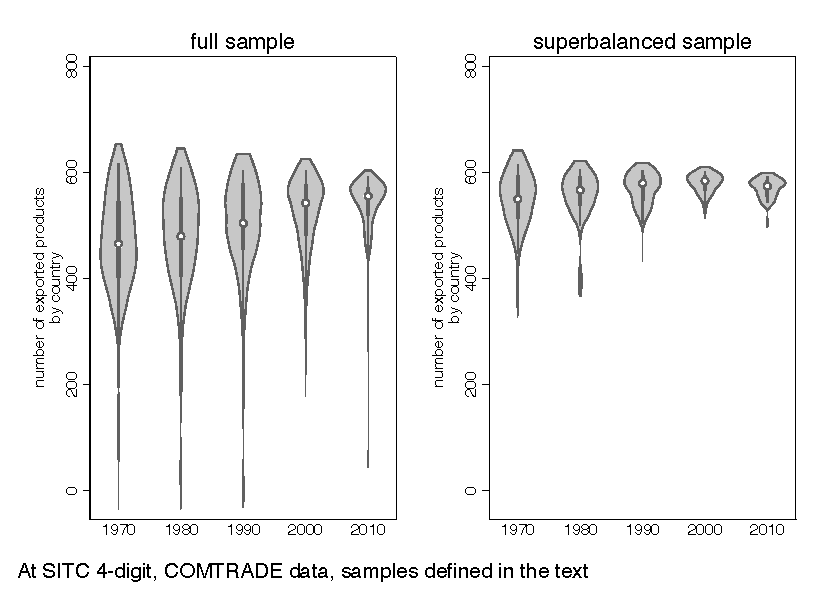
\includegraphics[trim = 0mm 0mm 0mm 0mm, clip, height=2.5in]{vioplot.pdf}}
	\end{center}
\end{figure}

Figures \ref{fig:vioplot} and \ref{fig:fall_of_sd} are the simplest way to make our point. 
The figures illustrate that an increasing number of countries exports a larger range of products, so that the export bundle of all countries is converging toward the entire range of goods.
The figures also illustrate that the increasing similarity of export bundles is robust to the examination of a more limited sample of exporters.\footnote{The full sample comprises all pairs. The superbalanced sample focuses on pairs which trade both ways in all years. See Appendix \ref{app:E}.} 
%The increasing similarity of product bundles corresponds to an increasing number of varieties of any given product that is available in the market. 
%A more densely populated product space may translate into an increase in the perceived substitutability of product varieties.

\begin{figure}[h!]
	\caption{Standard deviation in the number of products exported by each country \label{fig:fall_of_sd}}
	\begin{center}
		\setlength{\fboxrule}{1pt} %makes border lines thick
		\setlength{\fboxsep}{.1in} %increases distance to border
		\fbox{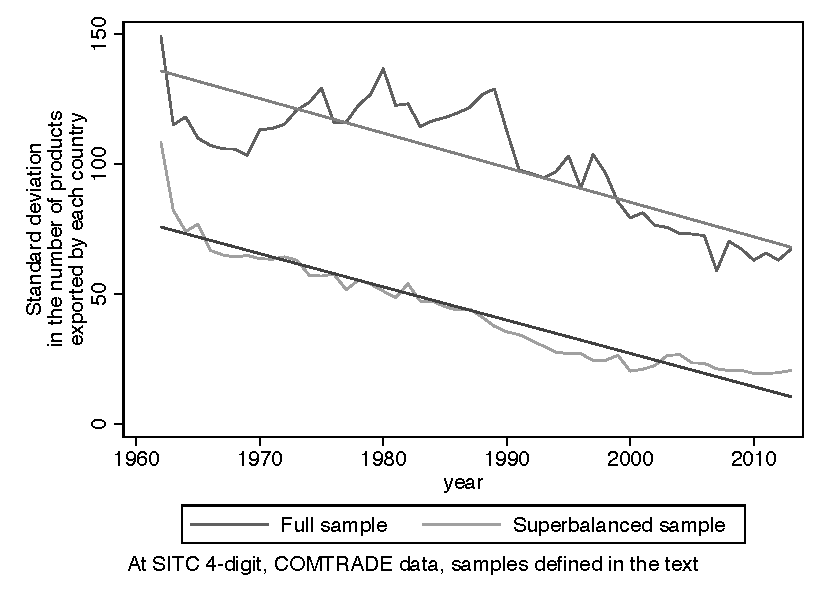
\includegraphics[trim = 0mm 0mm 0mm 0mm, clip, height=2.5in]{Fall_of_SD.pdf}}
	\end{center}
\end{figure}

We work with the canonical \cite{Anderson2003} framework to quantify the contribution of this mechanism. 
We find that the non-decreasing distance elasticity of trade can be explained by the increase in the perceived similarity of exporter-specific product bundles. 
%Limitation of our approach: we do not provide a model which delivers an endogenous increase in the price elasticity of demand b/c we want first to assess whether empirical evidence corroborates this explanation.
%Further work: verification in other frameworks how $\gamma$ or $\theta$ evolve and/or theoretical investigation.
One way to rationalize the evolution of the elasticity is to notice that the increasing similarity of product bundles means that more varieties of any given product are available in the market. 
A more densely populated product space may translate into a higher perceived substitutability of varieties of different national origin and result in higher measured substitutability of exporter-specific product bundles.

\subsection*{Prominent explanations of the distance puzzle}
%1.econometric approach; 2.trade cost function approach; next subsection: focus on trade elasticity and network approach (Chaney) + us
Recent work rationalizes the distance puzzle in three complementary ways: by pointing out a possible misspecification of the econometric model, by refining the specification of the trade cost function, and, more recently, through the lens of network analysis.

The first strand of the literature investigates the incidence of the estimation method on the distance puzzle.
\cite{SantosSilva2006} advocate estimating the gravity model in multiplicative form using a specific non-linear estimator, the Poisson Pseudo Maximum Likelihood (PPML).
Contrary to the canonical loglinear approach, this estimator provides consistent estimates and is robust to rounding error and overdispersion which are both likely features of trade data.\footnote{\cite{SantosSilva2011} and \cite{Fally2015} provide evidence on desirable properties of the PPML.
%Inadequacy of alternative non-linear estimators is discussed in \cite{Bosquet2015,Bosquet2014}.
\cite{Head2014} review properties of alternative estimators.
See also \cite{Bosquet2015,Bosquet2014}.}
The magnitude of the distance puzzle is reduced when the gravity model is estimated in multiplicative form (\cite{Bosquet2015, Head2013}).

%It is hence more accurate to state the puzzle as a non-decreasing distance elasticity of trade since the 1960s.
%SST2006 show that PPML is robust to measurement error in the underlying data (rounding of the data).
%SST2011 show that PPML remains consistent when zero trade flows are prevalent.
%The estimator is also robust to the misspecification of the conditional variance function.
%SST argue that PPML is unique in that it is consistent with non-count data, and is unit independent contrary to alternative non-linear estimators which seek to accomodate excessive variance (such as the negative binomial or the zip).
%because the trade equation in levels is subject to heteroskedasticity // because the conditional expectation of the loglinearized error term is not independent of the regressors // the assumption of conditional independence of the loglinearized error term does not usually hold.
%
%%Sensitivity of distance effect to estimation method is in two aspects: the level (lower in ppml) and the evolution (stable in ppml).
%%Main point is that ppml preferable to investigate magnitude of the distance puzzle b/c does not suffer from sample selection bias of ols: evolution exaggerated in ols b/c of the extensive margin of trade.
%In this paper we show an alternative way to account for this extensive margin of trade: importance of distance is decreasing for establishment of trade relations, while stable effect on existing trade relations (either through appendix using Egger et al.
%or through additional graph in paper using Egger et al.
%methodology).
%Together these facts illustrate that distance puzzle is a stable set phenomenon (this is main point of our part 1) - main point of part 2 is to document evolution of trade elasticity (show that this evolution is stronger in the stable set?).

The sensitivity of the distance puzzle to the estimation method is likely due to sample composition effects (\cite{Head2013,Larch2016}).
%PUT HERE REF TO ZIGNAGO-VICARD-MAYER: they argue that estimator puts different weights on big and small trade flows (not inconsistent)
%\cite{Head2013} show that the magnitude of the puzzle in the log-linear specification is reduced in the sample of stable trade partners.
Indeed, the growth of trade has been both intensive in the sense that the volume of established trade relations has increased and extensive in the sense that new trade relations have been established (\cite{Helpman2008, Baldwin2011}).
If trade relations have in priority been established between small and distant partners, the reduction in the number of zeros may have gradually reduced the underestimation of the distance coefficient in the loglinear specification.
\footnote{\cite{Larch2016} attribute the puzzle to the growing bias of the OLS estimates.
Using a nonlinear estimator and controlling for the number of exporting firms, they find a decreasing distance elasticity in 1980-2006.}
This explanation echoes \cite{Felbermayr2006} who pointed out that the log-linear specification was subject to sample selection bias due to the exclusion of zero trade flows.
They conjectured that the distance puzzle was an artefact of reduction in this bias through the extensive margin of trade.\footnote{This discussion leaves open the question of the estimator which correctly captures the level of the distance elasticity.
\cite{Head2013} argue that PPML gives little weight to small trade flows, characteristic of more distant partners.
For \cite{SantosSilva2006} small flows are more prone to measurement error.}
%\cite{Head2013} find that the level of the distance elasticity in the log-linear specification is reduced to the level of the non-linear estimate when the sample is restricted to partners predicted to have relatively big trade flows.
%They also show that the level of the distance elasticity increases when the PPML estimator is implemented on expenditure shares instead of trade volumes (\cite{EKS2012} method).
%%choice of estimator remains an open issue: if one believes that the main aspect of globalization is filling in of the zero trade matrix: new and small trade flows between relatively distant partners are key feature, then ppml may be inadequate because gives little weight to small flows.
%If however one believes that the main feature is the stability of the distance profile of trade, then the doubling of the distance elasticity of trade in the log-linear estimation appears suspicious and driven by fitting small trade flows.
%I construct the appendix on the distance profile of trade to argue that the ppml with stable elasticity conforms to the stability of the distance distribution of trade flows observed over 1963-2009.
%Our key point is to establish that the distance puzzle is a stable set phenomenon in ppml, and we seek to explain why trade in the stable set is not becoming less sensitive to distance: we deal with extensive margin by showing that distance plays less important role in formation of trade relationships.
%
%%misspecification of the trade cost function: non-monotonic relationship between transport costs and total costs, in particular through input-output relationships or, more simply, increasing importance of trade cost components other than freight costs/tariffs

The second and most prominent strand of the literature singles out the underpinnings of the trade cost function as key to understanding the distance puzzle.
The basic point formulated by \cite{Buch2004} is that the distance elasticity of trade is invariant to reductions in transportation and communication costs if their distribution over distance remains unchanged.\footnote{\cite{Egger2008} argues that the marginal effect of distance on trade is fundamentally non uniform across trade partners and decreasing in the level of bilateral trade.
This nonlinearity reinstates increased openness as a possible explanatory factor because a uniform reduction in trade costs has non uniform effects on bilateral trade.}
Furthermore, while the distance elasticity of transport costs may have decreased (\cite{Hummels2007}), other cost components, such as delays, may have become more distance-elastic (\cite{Hummels2013}).
More generally, as argued by \cite{Head2013}, if freight costs account for an ever smaller fraction of distance-dependent trade costs, the distance elasticity of trade will be determined by other, possibly persistent, cost components.\footnote{\cite{Head2013} propose a typology of persistent but unobserved trade costs.
\cite{Daudin2003, Daudin2005} put forward that trade costs may have remained stable as a share of value added.}
%
%%\cite{Egger2008} argues that the marginal effect of distance on trade is fundamentally non uniform across country pairs.
%It is decreasing in the level of bilateral trade, e.g.
%increasing in the toughness of competition in the destination and decreasing in the exporting capacity of the source.
%A reduction in the elasticity of trade costs to distance has non uniform effects on bilateral trade across country pairs and is compatible with an increasing distance elasticity of trade.
%%Egger combines issue of econometric misspecification of the gravity model and of theoretical explanation of increasing distance elasticity of trade as a consequence of increased openness.
%The main argument is that the loglinearity assumption in distance-trade relationship is flawed.
%He links misspecification of the estimated model and suggestion of a theoretical explanation for increasing marginal distance effects.
%The main point is that interaction effects of distance with characteristics of source and destination must be included on top of the standard fixed effects in estimating changes in marginal effect of distance to take into account average effect and distribution effect of changes in the distance elasticity of trade costs.
%The theoretical argument is about distance effect being a function of price indices (and therefore productivity and openness) and the number of varieties (population and productivity and openness).
%A given trade cost will matter more if the price index in the destination is lower and the number of varieties in source is lower b/c this reduces the volume of bilateral exports.
%According to Egger, the reduction in price indices in destination and of the number of varieties in the source explains the increase in the marginal effect of distance.
%Increased openness increases the toughness of competition in destination markets while decreasing the number of varieties exported by each source.
%But the impact of such changes on bilateral trade is non uniform across country pairs.
%When we take into account this distributional aspect, the marginal effect of distance on trade may increase.
%[conceptually this is similar to our argument: sensitivity to price differences increases, but works through different mechanism]  In terms of the econometric specification for the gravity model: interaction effects between country-specific variables and distance should be included on top of country fixed effects.

\cite{Krautheim2012} presents a complementary mechanism in the heterogeneous firms' framework.
He models the informational component of trade costs as a fixed cost which decreases in the number of exporting firms.
This refinement of the trade cost function magnifies the distance elasticity of trade because the number of exporters is decreasing in variable trade costs which increase with distance.
This magnification mechanism may have been reinforced by the increasing weight of information costs in total fixed costs.
%\cite{Krautheim2012} refines the specification of fixed trade costs in the heterogeneous firms' framework to rationalize the distance puzzle.
%The key assumption is that the informational component of fixed costs is decreasing in the number of exporting firms.
%As the number of exporters is decreasing in variable trade costs which increase with bilateral distance, this mechanism magnifies the elasticity of trade to distance.
%The magnification effect is enhanced if the informational component acquires greater weight, and results in an increasing distance elasticity of trade.
%The argument presented in \cite{Buch2004} is that a proportional reduction in trade costs would lead to increasing trade volumes and leave the distance distribution of trade unchanged.
%This suggests another explanation: the increasing importance of certain components of trade costs, such as trading on time, for most traded goods.

An alternative explanation put forward in models with input-output linkages is that the relationship between total trade costs and transport costs may be non-monotonic.
An increasing distance elasticity may be an endogenous outcome of transport cost reductions if they engender a reoptimization of the production process which ends up increasing the relative cost of long-distance trade.
One possible mechanism is trade cost magnification through multiple border crossings by goods as a consequence of increased production fragmentation (\cite{Yi2010,Daudin2011,Noguera2012}).
Another mechanism formalized by \cite{Duranton2008} works through quality upgrading.
Lower transport costs shift trade towards higher-quality inputs which are more distance-sensitive because their customization requires intensive communication, i.e.
more back-and-forth travelling, between upstream and downstream firms.
%in D&S transport cost reductions give incentive to input producers to increase quality of products, but higher quality means higher costs of technology transfer to downstream firm through back-and-forth travelling), hence total costs of trade increase.
%More distance sensitive because incurring higher total transaction costs which are magnified with distance through back-and-forth travelling: NOT more substitutable but increasingly customized (differentiated).
%Problem of D&S: the increase in distance elasticity is not generated within this mechanism, but rather by assuming standardized and customized goods, and showing that trade shifts towards customized goods which require technology transfer. D&S argue this is a within-sectoral mechanism.
%\cite{Berthelon2008} test the impact of the changing composition of world trade between 1985 and 2005 on the distance coefficient, but find that it has had a negligible effect.
%Berthelon and Freund find that 39\% of products and 54\% of trade has become more sensitive to distance over this period against 2.8\% of trade becoming less sensitive to distance.
%I don't cite Baldwin and Taglioni b/c they focus on  role of intermediates in correct specification of economic mass variables in gravity equation, but not discuss link between globalization and distance puzzle through intermediates.
%Whether transport costs have declined or increased, the crucial question for the evolution of the coefficient is whether non-distance dependent transport costs, such as loading costs at ports, have declined relatively to distance-dependent transport costs, such as fuel costs (\cite{Feyrer2009}).
%\footnote{\cite{Keller2013} find that the distance elasticity is increasing in the intensity of knowledge transfers required to produce a final good.} not cited b/c very different focus: Keller and Yeaple (2013) focus on sectoral differences in distance elasticity in cross-section to model trade between parent and affiliate as a function of product complexity, but complexity is very similar to intensity of communication in D&S.

\subsection*{A shift of focus to the trade elasticity}
%transition to our approach: heterogeneity matters (example: Chaney); our approach: investigation of product heterogeneity within canonical AvW approach
The focus of the literature on the shape of the trade cost function mirrors the expectation that the distance coefficient moves together with the elasticity of trade costs to distance.
But \cite{Chaney2018} provides a theoretical foundation for the gravity equation through the lens of network analysis which demonstrates that the distance coefficient can be invariant to the trade cost function.
In \cite{Chaney2018} the rate of distance decay in aggregate trade is linked to the rate of decay in the density of firms which cover that distance with their network of contacts.
As the geographic dispersion of the network is increasing in firm size, the shape parameter of the firm size distribution plays a key role in explaining movements in the distance coefficient.
Thus, technological advances in transportation increase the geographic dispersion of exports at the level of the firm \if 0 and enhance the degree of international production fragmentation \fi but have no incidence on the distance elasticity of aggregate trade as long as the stationary firm size distribution verifies Zipf's law.
 
%e.g. is such that the rank of the firm in terms of its weight in aggregate exports is inversely proportional to the frequency of such firms.
%In \cite{ChaneyThomas2018} the distance distribution of trade for any firm is determined by the location of its contacts.
%The trade cost function shapes the geographic dispersion of this network by affecting the probability of drawing a contact in each location at firm birth and subsequent network expansion through existing contacts.
%Network expands in two ways: acquiring contact for some cost; metting friends of your friends.
%The trade cost function determines the initial distribution of contacts, and hence affects probability of making a contact somewhere at any future date.
%However, I do not remember whether/how the trade cost function affects the cost of acquiring a contact in some location.
%The rate of distance decay in aggregate trade is driven by the rate of decay in the density of firms which cover that distance with their network.
%In the specific case in which the stationary size distribution verifies Zipf's law, e.g. is such that the rank of the firm in terms of its weight in aggregate exports is inversely proportional to the frequency of such firms, the distance elasticity takes a constant value\footnote{The distance elasticity equals $1+\epsilon$ where $\epsilon$ is a function of structural parameters.
%$\epsilon$ tends to 0 whenever the firm size distribution verifies Zipf's law.}.
%NB: distance elasticity is NOT equal to the shape parameter of the Pareto (which incidentally is 1 when firm size distribution follows Zipf's law.) Rather, the fact that the shape parameter equals 1 means that the distance coefficient is a constant (independent of changes in other structural parameters).
%BUT premise is that world cannot be flat for all firms: network must expand over distance with firm size.
%The empirical relevance of Zipf's law for the firm size distribution (\cite{Axtell2001,Gabaix2008,DiGiovanni2011}) would suffice to explain the stability of the distance coefficient.
%Structural changes in the trade cost function since the 1960s may have led to enhanced international production fragmentation and to increasing geographic dispersion of exports at the level of the firm.
%But such changes would have had no incidence on the value of the distance elasticity if the shape parameter of the firm size distribution had not deviated from one.
%Empirical evidence on the evolution of this parameter is insufficient to conclude on the validity of this theoretical mechanism.
%Nonetheless, the model highlights that an increasing distance elasticity is likely to reflect a change in the degree of firm heterogeneity.
 
%The model highlights that movements in the distance coefficient likely reflect changes in the degree of firm heterogeneity.
%I do not discuss directly the effect of enhanced fragmentation of production b/c already too much info.
%But basic idea is given by citing Chaney: shape of trade cost function will change extent of fragmentation but not necessarily the distance coefficient b/c evolution of heterogeneity is key.
%More generally argument of why GVC may be irrelevant is that effect may go both ways.
%If fragmentation arises as a consequence of lower trade costs, it is expected to increase the distance elasticity of trade through the magnification effect (more trade at closer distance) but also to decrease the distance elasticity of trade through enhanced technology transfer (product homogeneization): the two effects may be of similar magnitude.

The link between the distance coefficient and the parameter which captures the degree of structural heterogeneity in the economy is not specific to \cite{Chaney2018}.
Every theoretical foundation of the gravity model delivers a functional relationship of the distance elasticity with the intensity of the incentive to trade, 
i.e. the degree of structural heterogeneity in some model-specific dimension.
The combination of empirical evidence on the changing shape of the trade cost function with evidence on the stability of the distance distribution of trade indicates that structural heterogeneity may have contributed to the evolution of the distance coefficient.
However, empirical evidence on the evolution of structural heterogeneity in the economy since the 1960s is notoriously scarce (\cite{Head2013}).
%The structural interpretation of the trade elasticity depends on the micro foundations used to derive the gravity equation.
%In the canonical models this paper builds on it corresponds alternatively to the elasticity of substitution between country-specific composite goods, to the dispersion in productive efficiency across sectors, or to the intrasectoral dispersion in firm productivity.
%In all cases the trade elasticity is inversely linked to the degree of heterogeneity in a single model-specific dimension.

%Transition to our approach:  
We pursue the idea that a key parameter for understanding movements in the distance coefficient is the one measuring the degree of structural heterogeneity.
Following \cite{Arkolakis2012} we refer to this parameter as the `trade elasticity'.
%In theoretically derived gravity models of trade the value of the distance coefficient is not directly related to the level of trade costs.
%The level of trade costs, captured by country-specific fixed effects, influences the openness of each country.
%It is the product of two elasticities: the elasticity of trade flows to trade costs, and the elasticity of trade costs to distance.
%While the discussion on the distance puzzle in the literature has been mainly concerned with the evolution of the elasticity of trade costs to distance, one should look as well at the evolution of the elasticity of trade flows to trade costs.
%To effectively assess the evolution of structural heterogeneity in the economy since the 1960s we adopt an empirical approach.
%Instead of looking for a magnification mechanism inherent to the relationship of trade costs with distance, we investigate the evolution of the structural parameter which captures the intensity of the incentive to trade, e.g. the elasticity of trade flows to trade costs.
Because of data limitations inherent to our 60-year perspective, we can only estimate the trade elasticity in the Armington framework.
Structural heterogeneity is determined in this framework by perceived product substitutability, i.e.
the degree of product differentiation by place of origin.\footnote{This parameter plays no role in determining the trade elasticity in the Melitz-Chaney or Eaton and Kortum frameworks. The demand parameter comes back into the picture under alternative assumptions on the productivity distribution  (\cite{Bas2017}, \cite{Feenstra2018a}).}

%We assess the evolution of the trade elasticity in the canonical \cite{Anderson2003} framework in which structural heterogeneity captures the degree of product differentiation by place of production.
We estimate the distance elasticity of aggregate trade and the Armington elasticity of substitution between goods of different origin in each year between 1963 and 2013.
These two elasticities are identified separately.
We deduce the implied evolution of the elasticity of trade costs to distance from the two estimated elasticities.\footnote{\cite{Erkel-Rousse2002} do this exercise for just one point in time on a subsample of world trade flows.}
%The distance elasticity and the Armington elasticity are identified separately in the estimation while the elasticity of trade costs to distance is deduced from the estimated coefficients.
%We find robust evidence that the Armington elasticity has increased faster than the distance elasticity between 1962 and 2013.
%We conclude that the distance puzzle may be due to the increasing sensitivity of consumers to price differences.
%Further, we deduce the elasticity of trade costs to distance from the two estimated elasticities.
%We conclude that the evolution of the distance coefficient is compatible with a decreasing sensitivity of trade costs to distance.
Our main result is that the increase in the Armington elasticity not only rationalizes the non-decreasing distance elasticity of trade but also hints at a reduction in the elasticity of trade costs to distance.
We conclude that in the Armington framework the distance puzzle is fully explained by the increasing sensitivity of consumers to price differences.
More generally, our results suggest that the distance puzzle may be due to a reduction in structural heterogeneity.

%COMPLEMENTARITY OF RESULTS TO PREVIOUS STUDIES
%our approach differs and complements previous findings: not differentiation of varieties linked to consumer taste heterogeneity, but rather degree of similarity of the product mix.
%Underline consistency of our results with B\&F and differentiate directly from B\&W b/c aggregate rather than sectoral approach
To the best of our knowledge, \cite{Berthelon2008} is the only paper that studies the impact of changes in perceived product substitutability on the distance coefficient.
Using estimates of sectoral Armington elasticities obtained by \cite{Broda2006}, \cite{Berthelon2008} find a positive relationship between the variation in sectoral distance coefficients and the variation in Armington elasticities between 1985-1989 and 2001-2005.\footnote{\cite{Berthelon2008} work with 776 sectors defined at the SITC Rev.2 4-digit level.
\cite{Broda2006} use time-series variation in prices and market shares for the set of exporters to the US market to get one value for the Armington elasticity in 1972-1988 and another value in 1990-2001.}
%\cite{Berthelon2008} also investigate the evolution of the elasticity of trade costs to distance using data on transport costs and tariffs, and conclude that this elasticity is likely to have decreased.
%\cite{Berthelon2008} use average bilateral sectoral trade flows in each five-year period.
Our approach is different from \cite{Berthelon2008} because we focus on the aggregate Armington elasticity and provide direct estimates of this parameter in each year between 1963 and 2013.
Our approach is different from \cite{Broda2006} because we exploit cross-sectional variation in prices and trade shares to infer the extent of substitutability while these authors exploit changes in prices and trade shares over time to identify one point estimate.
Our approach enables us to trace out changes in the perceived similarity of the product mix that countries supply to the world market.
%\footnote{Our approach differs from \cite{Broda2006} because we exploit cross-sectional variation in prices and trade shares to infer the extent of substitutability while these authors use time variation to identify one point estimate.}
%Difference with Broda and Weinstein is not only sectoral vs. aggregate but also the choice of using cross-sectional differences in trade shares owning to the cross-sectional variation in prices to infer the extent of substitutability.

We proceed in three steps.
First, we examine the hypothesis that the distance puzzle is a by-product of compositional changes in the set of traded goods or of trading pairs.
We refute this hypothesis by showing that the distance puzzle is more pronounced in the stable set.
%We start with invalidating the hypothesis that the distance puzzle is a by-product of compositional changes in the set of trading pairs or in the set of traded goods.
%We estimate the gravity model in multiplicative form while fixing the weight of each sector in total trade and restricting the set of partners to reciprocally active trade relationships in each year of the sample.
%The increase in the distance elasticity is magnified in this stable set.
%This result is consistent with \cite{Berthelon2008} who find that sectoral distance elasticities are more likely to have increased for homogeneous goods.
%As the share of homogeneous goods has decreased in total trade, fixing trade shares helps preserve the importance of homogeneous goods: therefore magnification of distance puzzle in stable set.
%The distance puzzle is a stable set phenomenon.

Second, we point out that a straightforward nonlinear estimation approach allows identifying the aggregate Armington elasticity in cross-section. The key intuition follows \cite{Imbs2015} who show that a consistent estimate of the aggregate elasticity is obtained on sectoral data by constraining sectoral elasticities to equality in the estimation.\footnote{The focus of \cite{Imbs2015} is on documenting the heterogeneity bias, i.e. that the estimated aggregate elasticity differs from the `true' elasticity defined as the weighted average of the sectoral parameters. 
Our focus is on obtaining an estimate consistent with the aggregate trade data.} But our estimation approach differs from \cite{Imbs2015} - who generalize \cite{Feenstra1994} - in that these authors identify the elasticity while using the variation in relative prices and market shares over time while we relax the assumption of parameter invariance and work with subsequent cross-sections. 

Third, we use non linear least squares on pooled sectoral data aggregated in a theoretically sound way to provide estimates of the Armington elasticity in each year between 1963 and 2013.
We then carry out a series of robustness checks to deal with missing unit values, zero trade flows, low data quality and endogeneity.
We document an increase of between 22\% and 60\% of the Armington elasticity.  
%In the estimation we instrument unit values - our proxy of prices - with lagged unit values together with the lagged real exchange rates specific to each bilateral relationship to address endogeneity concerns.
%Second, we use the assumption that consumer preferences are well represented by a two-tier CES utility function, e.g. within sectors between country-specific varieties at the lower level and between sectoral composite goods at the upper level, to consistently aggregate sectoral price information and construct the landed price of the composite good that each source delivers to each destination relatively to the price of the composite good the importer acquires from the world.
%This allows direct estimation of the annual aggregate price elasticity of demand across country-specific composite goods for the full set of bilateral trade relationships.
%This elasticity is the structural parameter which determines the elasticity of trade flows to trade costs in the canonical \cite{Anderson2003} framework.
%the consistent aggregation procedure given by the two-tier preference structure of the Armington model to construct the relative price of the composite good which each source exports to each destination.
%Third, we present our results for the aggregate Armington elasticity.
%Third, we present the results of this method and conduct a number of robustness checks.
%We discuss the bias introduced by the presence of zero trade flows.


Finally, we discuss the implications of the increasing Armington elasticity for the distance puzzle. 
%The distance elasticity and the Armington elasticity are identified separately in the estimation.
%, while the elasticity of trade costs to distance is deduced from the estimated coefficients.
The Armington elasticity has increased faster than the distance elasticity of aggregate trade between 1963 and 2013.
The evolution of the distance coefficient is thus compatible with a reduction of the elasticity of trade costs to distance.

%This allows direct estimation of the annual aggregate price elasticity of demand across country-specific composite goods for the full set of bilateral trade relationships.
%This elasticity is the structural parameter which determines the elasticity of trade flows to trade costs in the canonical \cite{Anderson2003} framework.


%We address endogeneity concerns which stem from the presence of zero trade flows in two complementary ways.
%In the first specification observed prices are instrumented with the real exchange rate which is specific to each bilateral relationship.
%In the second specification we use the prediction of the model that conditional on destination-specific characteristics and bilateral trade frictions, the frequency of zero trade flows carries information on fundamental exporter ability to construct an instrument which identifies substitutability on the basis of cross-sectional variation in exporter-specific prices on the world market.
%The distance elasticity and the trade elasticity are identified separately in the estimation, while the elasticity of trade costs to distance is deduced from the estimated coefficients.
% We find robust empirical evidence that this elasticity has increased faster than the distance elasticity of aggregate trade between 1963 and 2009.
%We discuss our main result on the 13\% increase in the aggregate trade elasticity between 1963 and 2009 in light of the distance puzzle and report a series of robustness checks.

%is endogeneity a big concern at the level of aggregate bundles? if demand shocks lead to movement up the supply curve within each sector, reasonable to assume that wash out across sectors?
%DISCUSS GENERALITY OF RESULTS EITHER HERE OR IN PART 3: Although we document reduction in heterogeneity in the Armington framework, our results likely to be more general.
%If zeros are a statistical feature and given that sectoral Armington elasticities are finite, reduction in nb of zeros means that domestic price of the good has decreased enough for the volume of trade to increase sufficiently in order to be recorded in trade statistics.
%Hence, dispersion in prices of domestically produced goods decreases overtime.
%In Ricardian framework this is equivalent to reduction in dispersion of technological ability, e.g. a reduction in the strength of comparative advantage or an increase in the Ricardian trade elasticity.
%Evidence of this is provided in Levchenko and Zhang.
%As documented in L\&Z, strong heterogeneity across countries: in certain countries no reduction in dispersion.
%This could explain muted evolution of aggregate trade elasticity in our sample (additional robustness check would consist in verifying that increase in trade elasticity is magnified in the superbalanced sample and/or for the fixed set of goods).

\section{The magnitude of the distance puzzle} \label{sec:part1} 
%REVISION: we adopt same notation as HM2013: distance effect is $\delta=-\epsilon\rho$; we adopt same scale on all figures and update figures to 1962-2013; we also reformulate table for summary effects (no FTA)
%NOT DONE: explain why we always estimate gravity model for aggregate trade; improve discussion of fta effect and include discussion of fixing distance distribution of trade (not intensification of within-FTA trade through relative reduction in cost of within-FTA trade but broadening of FTA coverage (extensive margin))
In this section we evaluate the sensitivity of the distance puzzle to compositional changes in the set of traded goods and in the set of trading pairs over 1962-2013.
Such changes were identified in previous estimations of the loglinearized gravity model as explanatory of movements in the distance coefficient.\footnote{\cite{Berthelon2008} find that changes in the sectoral composition of world trade do not help to explain movements in the distance coefficient in 1985-2005.
\cite{Head2013} find that the distance puzzle is reduced in the set of stable pairs between 1960 and 2005 when the model is estimated in loglinear form.}
We estimate the gravity model in multiplicative form and document that the distance puzzle is magnified in the sample of stable pairs and robust to fixing the sectoral composition of world trade.


%REMOVED PART ON FTA: We also check whether the conduct of trade policy helps rationalize the distance puzzle.
%If Free Trade Agreements (FTAs) reduce the relative cost of within-FTA trade and FTA formation takes place at short-distance, regional integration would result in an increasing intensity of within-FTA trade, and mechanically induce an increasing distance elasticity of trade costs.
%We fail to find supportive evidence of this hypothesis in the data.
%Adopting a more flexible approach than \cite{Bosquet2015} in allowing the FTA effect to vary overtime we find weak evidence of trade intensification through FTA formation.
%This mechanism does not help explain the distance puzzle in the full sample.
%Rather, the process of regional integration appears to have been working through the extensive margin, e.g. through the increasing geographic scope of FTAs and their increasing coverage of short-distance trade.
%We do not observe directly the shape of the trade cost function.
%We know from previous studies that the transport cost component is unlikely to be key.
%Hence focus on institutional component b/c NTB and information costs may be key.
%These results motivate our focus on structural heterogeneity as a possible alternative driving force behind the non-decreasing distance elasticity of trade.
 
\subsection{Baseline estimate of the distance puzzle} \label{subsec:baselineDP}
We use the COMTRADE dataset to make our investigation of the distance puzzle directly comparable to \cite{Head2013} and \cite{Berthelon2008}.
We work with the 4-digit SITC Rev.1 product classification (600-700 goods) because it provides the longest and most comprehensive coverage of disaggregate bilateral trade (1962-2013).
%We stop short of 2014-2015 where data is subject to revision.
%The earliest available year is 1962.
%We focus on 1965-2011 for consistency with the timeframe used in estimation of Armington trade elasticities in section \ref{sec:part3}.
Data on bilateral distance, bilateral trade cost controls such as adjacency, common language, colonial linkages, and data on belonging or having once belonged to the same country are taken from the CEPII.\footnote{See \cite{Mayer2011}
	The database is available at \url{www.cepii.fr}.
	We constructed bilateral distance and bilateral cost controls for East and West Germany, USSR, and Czechoslovakia.}


We conduct the estimation on CIF import flows.
We restrict the sample to trade in goods which are attributed to specific 4-digit categories and to pairs for which we have data on bilateral trade cost controls.
App.
\ref{app:E} lists the resulting set of countries.
For each active pair attributed sectoral flows are summed to obtain total bilateral trade.
We refer to the resulting sample as `the full sample'.
It covers between 88\% and 99\% of reported trade in COMTRADE.
%\footnote{COMTRADE itself covers between 70\% and 90\% of total world merchandise trade according to the WTO (\url{http://stat.wto.org/Home/WSDBHome.aspx}).} 
%Our dataset covers between 70\% to 90\% of total world merchandise trade according to the WTO.\footnote{See \url{http://stat.wto.org/Home/WSDBHome.aspx}, accessed in May 2011.}.
%More precisely, 70\% in 1962, this increases to 80\% in the 1960s, stays stable until the late 1980s, and then increases to approximately 90\% in the 1990s and 2000s.
%As trade data is of better quality for imports, the estimation is conducted on import flows.

We follow the canonical \cite{Anderson2003} derivation of the gravity model to express aggregate bilateral trade $X_{ij}$ as a function of bilateral trade barriers $\tau_{ij}$, multilateral trade resistance terms in source $i$ and destination $j$ (resp.
$\Pi_{i}$ and $P_{j}$), and nominal incomes $Y_{n}$ with $n\in\left\{i,j,w\right\}$ where $w$ is world income.
\footnote{This formulation is not specific to the Armington framework.
See footnote 20 in \cite{Eaton2002} and subsequent discussions of equivalence in  \cite{Arkolakis2012, Head2013}.}


\begin{eqnarray}
X_{ijt} & = & \left(\frac{Y_{it}Y_{jt}}{Y_wt}\right)\left(\frac{\tau_{ijt}}{\Pi_{it}P_{jt}}\right)^{\epsilon_t}\label{eqn:1}
\end{eqnarray}
%$X_{ij,t}$ is the value of goods from country $i$ consumed in country $j$ in year $t$, i.e. bilateral imports at cif prices.
%Imports are a function of the nominal income of each trading partner $Y_{ij,t}$ and $Y_{j,t}$, of world income $Y_t$, of bilateral trade costs $\tau_{ij,t}$, and of inward and outward multilateral trade resistance terms $P_{j,t}$, $\Pi_{i,t}$.
%\footnote{$\Pi_{i}$, $P_{j}$ are respectively inward and outward MR terms.} 

We include the time subscript $t$ not only on each variable but also on the elasticity of trade flows to trade costs $\epsilon$ to underline that this parameter is subject to change.
In the Armington framework $\epsilon_t=1-\sigma_t$ where $\sigma_t$ corresponds to the elasticity of substitution between goods of different national origin.
We seek to quantify the evolution of the elasticity of aggregate trade flows to trade costs.
Hence, the key parameter of interest for this paper is the Armington elasticity which captures perceived substitutability of composite goods which differ by their place of production.


As total bilateral trade costs $\tau_{ijt}$ are not directly observed for each pair and year, we model them as a function of observable time-invariant bilateral controls which are distance, adjacency, and common language together with persistent but time-varying controls standard in the gravity literature which are historical and current colonial linkages as well as belonging or having once belonged to the same country.
We include an unobserved bilateral trade cost component $\nu_{ijt}$ assumed to have mean zero conditional on the observables.
\footnote{\if 0 This assumption can be questioned, in particular with respect to excluded trade cost controls which vary as a result of trade policy decisions.
	\fi The error term contains bilateral variation in trade costs due to trade policy.
	The question of possible changes in the distance distribution of trade costs as a consequence of policy decisions is beyond the scope of this paper.}
%For consistency it would be good to redefine colonial linkages and same country as time-invariant controls: group 'having been /currently are' as single variable.
%and a vector $Z_2$ of trade cost controls linked to trade policy such as common membership of GATT/WTO and common membership of an FTA.
We denote distance $\eth_{ij}$, group the other time-invariant observables in the vector $Z$ and time-varying observables in the vector $S_t$ to get the following specification of the trade cost function:
\begin{eqnarray}
\tau_{ijt}&=&\exp\left\{\rho_t\ln{\eth_{ij}}+{Z}'\zeta_{t}+{S_t}'\varsigma_{t}+\nu_{ijt}\right\} \label{eqn:20}
\end{eqnarray}
%\begin{eqnarray}
%\tau_{ij,t}&=&exp\left\{\rho_t\ln{dist_{ij}}+%{Z_{1,t}}'\beta_{1,t}+{Z_{2,t}}'\beta_{2,t}\right\} \label{eqn:20}
%\end{eqnarray}

Replacing (\ref{eqn:20}) in (\ref{eqn:1}), substituting source and destination specific variables with country fixed effects (resp.
$f_{it}$ and $f_{jt}$), defining a constant $\xi_t$ and specifying a multiplicative error term $\xi_{ijt}$ which includes the exponentiated unobserved bilateral trade cost gives the equation to be estimated on aggregate bilateral trade: 
\begin{eqnarray}
X_{ijt}&=&\exp{\left(\xi_t-\delta_{t}\ln{\eth_{ij}}+{Z}'\zeta_t+{S_t}'\varsigma_t+f_{it}+f_{jt}\right)\xi_{ijt}} \label{eqn:4}
\end{eqnarray}
%\begin{eqnarray}
%X_{ij}&=&\exp{\left(\alpha_0-\alpha_1\ln{\eth_{ij}}+{Z}'\beta_1+{Z_2}'\beta_2+fe_{exp}+fe_{imp}\right)\epsilon_{ij}} \label{eqn:4}
%\end{eqnarray}
%where $fe_{exp}$ and $fe_{imp}$ are respectively exporter and importer fixed effects and $\xi_{ij}$ is a multiplicative error term which includes the unobserved bilateral trade cost.


To ensure consistency of the point estimates we do not loglinearize the model although switching to a non-linear estimator may entail a loss of efficiency (\cite{Manning1999}).
We implement (\ref{eqn:4}) in the full and superbalanced samples using the PPML estimator (\cite{SantosSilva2006}).
The estimation is conducted in cross section.
The parameter of interest is the distance elasticity, $-\delta_t$, which corresponds to the product of the distance elasticity of trade costs $\rho_t$ and of the trade elasticity $\epsilon_t$.
\footnote{We follow the notation in \cite{Head2013} (see equation (4), p.1205).}


%graph updated to 1962-2013
\begin{figure}[h!]
	\caption{Baseline estimate of the distance puzzle \label{fig:DP_baseline}}
	\begin{center}
		\setlength{\fboxrule}{1pt} %makes border lines thick
		\setlength{\fboxsep}{.1in} %increases distance to border
		\fbox{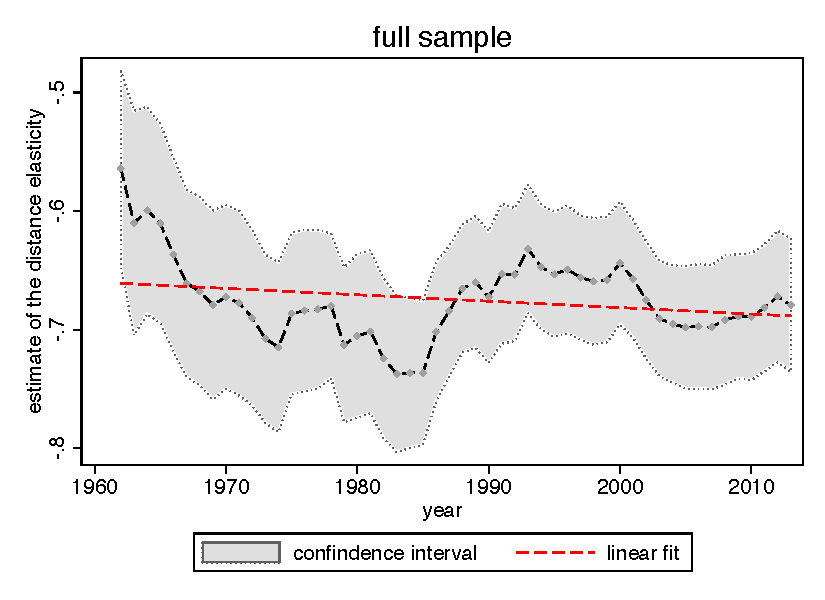
\includegraphics[trim = 0mm 0mm 0mm 9.5mm, clip, height=2.5in]{DP_baseline.pdf}}
	\end{center}
\end{figure}

Figure \ref{fig:DP_baseline} gives the results.
In the full sample (left pane) the distance effect $\delta_t$ increased by $4.5$\% between 1962-2013 (left pane), but this increase is only marginally significant.
Consistently with previous studies we find that the distance sensitivity of trade has not been reduced over time.
We obtain the large confidence intervals shown in Figure \ref{fig:DP_baseline} when we implement the Huber-White correction of standard errors.
\footnote{Switching to the panel approach with the full set of country-year dummies does not achieve significant improvement in precision.}
Standard errors are reduced by an order of magnitude when this correction is not implemented. 
%\cite{SantosSilva2006} advocate this approach to account for possible misspecification of the conditional variance function.
%Computing heteroskedasticity-robust standard errors yields the large confidence intervals shown in Figure \ref{fig:compsample}, putting in doubt even the existence of the distance puzzle
%The loss of precision is due to computing heteroskedasticity robust standard errors \if 0 implementing the Huber-White correction of standard errors advocated by \cite{SantosSilva2006} \fi to account for possible misspecification of the conditional variance function.
Considering that the PPML approach already takes into account heteroskedasticity, and that we are looking at these point estimates as if they were descriptive statistics on the whole population, we take the results shown in Figure \ref{fig:DP_baseline} as sufficient evidence for the existence of the distance puzzle. 

Still, the decrease in the absolute value of the estimated distance elasticity from the mid 1980s to the early 1990s is suspiciously concomitant with the entry of new countries in the dataset following the fall of the Soviet Bloc. The next section studies the potential effect of that change in sample.

\subsection{The magnitude of the sample composition effect} \label{subsec:data}

Figure \ref{fig:active_pairs} summarizes the main features of the country coverage of the data.
The number of active pairs increases more than fourfold in 1962-2013 (in dash, left scale), both because more countries report trade to COMTRADE and because more pairs have non-zero trade flows (\cite{Helpman2008}).
Active pairs make up between 45\% and 73\% of the total number of possible trade relationships, with a clear upward trend (in red, right scale).

%graph updated for 1962-2013
\begin{figure}[h!]
\caption{Active pairs in COMTRADE (1962-2013) \label{fig:active_pairs}}
\begin{center}
\setlength{\fboxrule}{1pt} %makes border lines thick
\setlength{\fboxsep}{.1in} %increases distance to border
\fbox{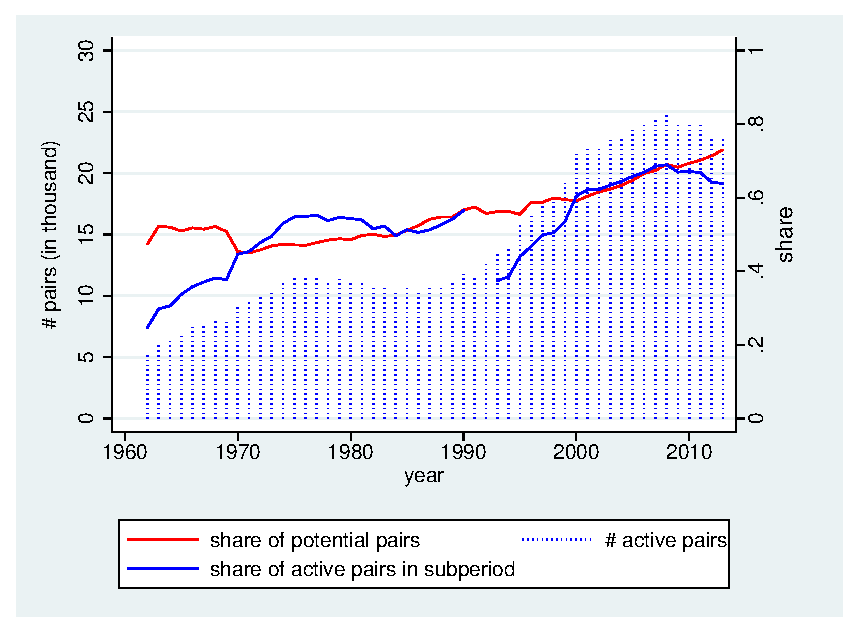
\includegraphics[height=2.5in]{part1_active_pairs.eps}}
\end{center}
\end{figure}

If we focus on the set of pairs that report non-zero trade in at least one year, the share of active pairs increases by 22 percentage points between 1962 and 1990 and by 27 percentage points between 1993 and 2013 (in blue, right scale).
\footnote{We split the sample in two subperiods, 1962-1990 and 1993-2013, to take into account country creation and disappearance in the early 1990s.}
By the end of the sample about 2/3 of pairs which trade at least once between 1962 and 2013 are reporting non-zero trade.


Hence, sample composition effects are substantial.
Nonetheless, the bulk of total trade is attributable to the 786 pairs which trade both ways in every year.
We refer to this set of stable reciprocal pairs as the `superbalanced' sample and use it to investigate the magnitude of the sample composition effect.
\footnote{The superbalanced sample includes 32 countries listed in App. \ref{app:E}. The appendix discusses trade coverage.\label{fnsuperbalanced}}


In the superbalanced sample (right pane) the increase in the distance effect $\delta_t$ is magnified to $18.2$\%, and this increase is strongly significant.\footnote{The annualized growth rate is 0.09\% in the full sample and 0.33\% in the superbalanced sample.}
%The distance elasticity is clearly non-decreasing, and this finding holds in the set of stable partners.
Moreover, the distance puzzle is exacerbated in the sample of stable trade relationships.\footnote{The opposite result holds in the loglinear specification (\cite{Head2013})
In OLS the decrease in the distance elasticity due to the elimination of small trade flows between distant partners trumps the increase in the distance elasticity of stable trade relationships.}
We take the results shown in Figure \ref{fig:compsample} as more evidence for the existence of the distance puzzle. 

%graph updated to 1962-2013
\begin{figure}[h!]
	\caption{Sample composition effect on the distance puzzle\label{fig:compsample}}
	\begin{center}
		\setlength{\fboxrule}{1pt} %makes border lines thick
		\setlength{\fboxsep}{.1in} %increases distance to border
		\fbox{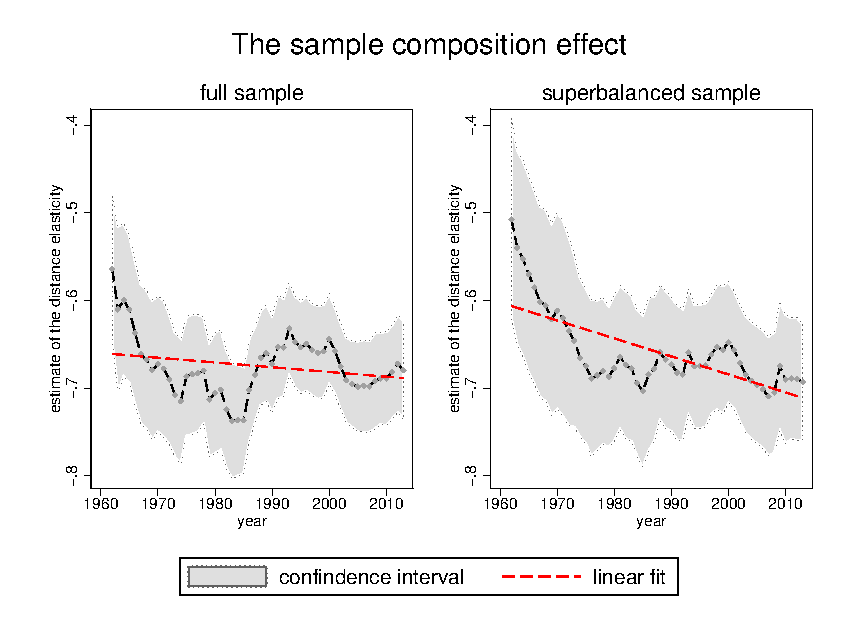
\includegraphics[trim = 0mm 0mm 0mm 9.5mm, clip, height=2.5in]{sample_composition_effect_1962.eps}}
	\end{center}
\end{figure}



\subsection{The magnitude of sectoral composition effects} \label{subsec:robustpuzzle}
Next, we demonstrate that the distance puzzle is robust to product composition effects.
In particular, the non-linearity in the evolution of the distance coefficient \if 0 is reduced in the sample of stable pairs (Figure \ref{fig:compsample}), and it \fi disappears once we control for product composition effects (see Figure \ref{fig:compbundle} below).

We assess the incidence of sectoral composition effects in two ways.
The first exercise consists in fixing the sectoral composition of world trade.
The second exercise consists in fixing the sectoral composition of the bundle supplied by each exporter to the world market.

%The intuition is that according to the model there should be substitution away from sectors which experience elasticity increases.
%Hence, muted puzzle?
%Each exercise consists in implementing a specific reweighting procedure.

In the first exercise we fix the sectoral composition of total trade to the initial year of the sample.
%we fix the share of each sector in total world trade to its share in the initial year of the sample.
Denoting each 4-digit sector $k$ and the annual share of the sector in world trade ($w,t$) by $s^{k}_{w,t}$, the reweighting procedure fixes the share of each 4-digit sector in world trade to its share in 1962.
The reweighted sectoral bilateral flow is $\tilde{X}^k_{ijt}=X^k_{ijt}*\frac{s^k_{w,1962}}{s^k_{w,t}}$.
The reweighted sectoral flows are summed for each pair, and the gravity equation is estimated in each year for aggregate bilateral trade.


Results are shown in Figure \ref{fig:compworld}.
\if 0 The non-linearity in the evolution of the distance coefficient is substantially reduced in the full sample (left pane),\fi The evolution of the distance coefficient becomes much more linear in the full sample (left pane), and this exacerbates the distance puzzle to a 14.5\% increase in $\delta_t$.
The impact of this reweighting procedure is about nil in the sample of stable pairs (right pane) where $\delta_t$ increases by 18.4\%.\footnote{The annualized growth rate is 0.26(0.33)\% in the full (superbalanced) sample.
Confidence intervals are reported for the Huber-White correction of standard errors.
Without it standard errors are reduced by a factor of 10.}
Indeed, the main incidence of fixing the sectoral composition of world trade is the elimination of short-term fluctuations in the distance coefficient due to fluctuations in the weight of the energy sector.
As this sector plays a relatively minor role in trade of stable reciprocal partners, the reweighting procedure has little incidence on the distribution of trade over distance in this sample.
%\footnote{Results on the incidence of the energy sector on the distance puzzle are available upon request.}.

%graph updated for 1962-2013
\begin{figure}[h!]
\caption{Product composition effect: fixing the world bundle  \label{fig:compworld}}
\begin{center}
\setlength{\fboxrule}{1pt} %makes border lines thick
\setlength{\fboxsep}{.1in} %increases distance to border
\fbox{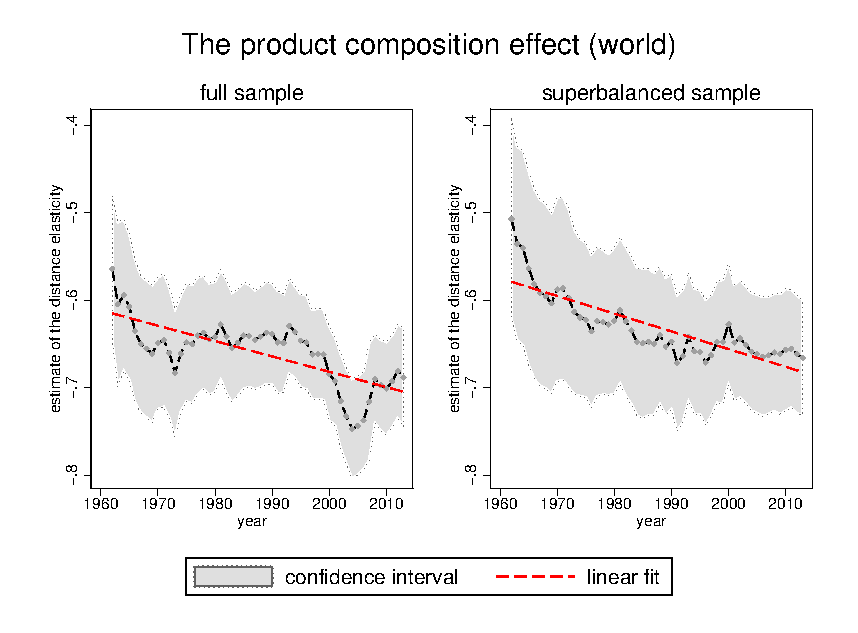
\includegraphics[trim = 0mm 0mm 0mm 9.5mm, clip, height=2.5in]{product_composition_effect_world_1962.eps}}
\end{center}
\end{figure}

%This exercise is only possible for countries that exist as partners (!) in 1962, so sample only includes countries that are listed as partners by reporters that exist in 1962
In the second exercise we fix the composition of the bundle supplied by each exporter $i$ to the world market.
Denoting the annual share of the sector in world imports from $i$ by $s^{k}_{i,t}$, the reweighting fixes the share of each 4-digit sector in world imports from $i$ to its share in 1962.
The reweighted sectoral bilateral flow is $\tilde{X}^k_{ijt}=X^k_{ijt}*\frac{s^k_{i,1962}}{s^k_{i,t}}$.
The resulting sectoral flows are summed for each pair, and the gravity equation is estimated on total reweighted bilateral trade.
%This investigation is complementary to \cite{Berthelon2008} who find that changes in the relative weight of products in 1985-2005 are not explanatory of movements in the distance coefficient.
 

%graph updated for 1962-2013
\begin{figure}[h!]
\caption{Product composition effect: fixing the country bundle  \label{fig:compbundle}}
\begin{center}
\setlength{\fboxrule}{1pt} %makes border lines thick
\setlength{\fboxsep}{.1in} %increases distance to border
\fbox{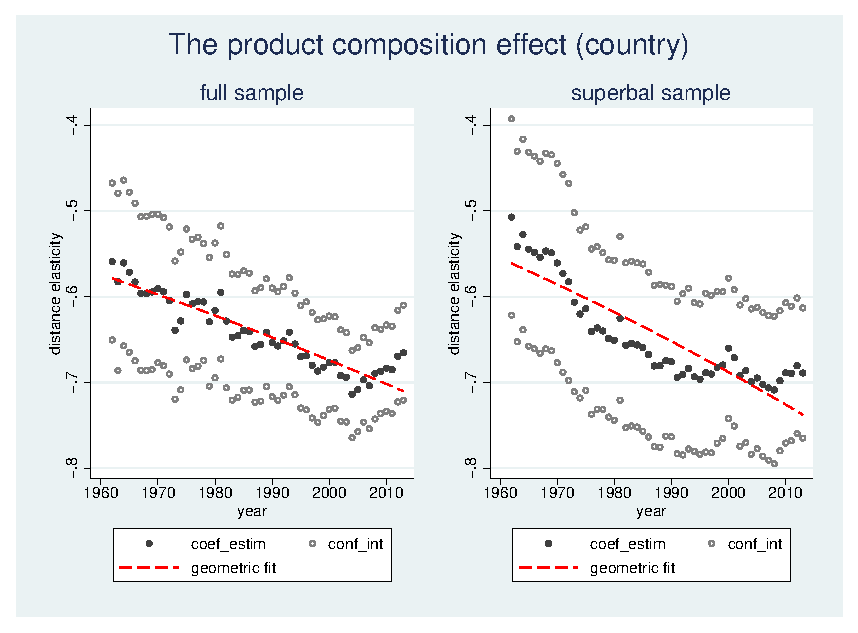
\includegraphics[trim = 0mm 0mm 0mm 9.5mm, clip, height=2.6in]{product_composition_effect_country_1962.eps}}
\end{center}
\end{figure}

As illustrated in Figure \ref{fig:compbundle}, fixing the composition of the country-specific composite good \if 0 eliminates the non-linearity in the evolution of the distance coefficient and \fi
exacerbates the magnitude of the distance puzzle.
%\footnote{This is consistent with \cite{Berthelon2008} who find that products initially perceived as more homogeneous are more likely to have experienced an increase in the distance elasticity. Applying the \cite{Rauch1999} classification we find that the share of differentiated goods in total trade has increased by almost 20 percentage points (from 42 to 60\% of total trade in 1962-2000).}.

Further, while the degree of precision in the estimation of the gravity equation with the Huber-White correction of standard errors remains similar to the benchmark specification, 87\% of the variation in the distance coefficient is attributable to the time trend in the full sample, against just 7\% in the benchmark specification.
\footnote{In the superbalanced sample 77\% of the variation is attributable to the time trend when the product bundle is fixed against 49\% when the product bundle is not fixed.}
The corresponding annualized growth rate is .40\% in the full, and .54\% in the stable sample.
This corresponds to a 22.7\% increase in the distance sensitivity of trade between 1962 and 2013 in the full sample, and to a 31.4\% increase in the sample of stable pairs.

We conclude that short-term fluctuations in the distance effect $\delta_t$ are likely attributable to product and sample composition effects.
But the long-term evolution of the distance effect appears linked to structural changes.
These structural changes are more pronounced in the set of stable trade relationships.

%this pattern is reinforced in the set of stable trade relationships.
%The superbalanced sample is a rectangular sample which includes 32 countries: Argentina, Belgium-Luxembourg, Brazil, Canada, Chile, Colombia, Denmark, France, Germany, Great Britain, Greece, Hong Kong, Iceland, Israel, Italy, Japan, Malaysia, Mexico, Netherlands, Philippines, Portugal, Paraguay, Singapor, South Korea, Spain, Sweden, Switzerland, Thailand, Tunisia, Turkey, Venezuela and the USA.
%China, India, Sub-Saharan African, Central and Eastern European countries do not have a reciprocal trading relationship in all years with any single country, and are thus excluded.

\if 0
%this subsection is discarded b/c FTA database not updated in 2009-2013 (should be updated in 2006-2013...)
%\subsection{The magnitude of the FTA effect} \label{subsec:distdistrib}
%FTA formation and the relative intensity of within-FTA trade
%Position this section as complementary to Hummels who investigates elasticity of transport costs to distance, B\&F who investigate incidence of changes in tariffs on distance, and us who analyze reduction in institutional costs.
Differentiate approach from B\&B by showing that we estimate naive effect and then decompose what is due to extensive margin from `true' FTA effect: distance puzzle magnified.
We consider the possibility that structural changes affected the distance distribution of trade costs inducing an increase in the distance elasticity.
The distance elasticity of transport costs is likely to have decreased since the 1960s (\cite{Hummels2007}, \cite{Berthelon2008}).
The distance elasticity of ad valorem tariffs is also unlikely to have increased (\cite{Berthelon2008}).
However, institutional and informational trade barriers may have been disproportionately reduced for within-FTA trade and may have resulted in the intensification of short-distance trade if FTAs have predominantly consisted in intraregional integration.

%if local trade costs decrease faster than long-distance trade costs (which shows up as regionalization), then we pick up an increasing distance elasticity of trade b/c the measured elasticity of trade costs to distance would increase due to assumption of loglinear relationship (misspecification).
Measure this with formation of FTAs: not just reduction in tariffs but also in associated NTBs: standards, hurdles, information costs.


\cite{Bosquet2015} investigate the impact of FTA formation on the distance puzzle while controlling for the endogeneity of country selection into FTAs with the \cite{Baier2007} methodology.
Constraining the trade creating effect of FTAs to be identical in each year and for all FTAs, \cite{Bosquet2015} find that FTAs have had no impact on the evolution of the distance elasticity.
This result may seem puzzling because the trade-creating effect of FTAs is expected to be reinforced by controlling for endogenous selection (\cite{Baier2007}, \cite{Egger2011}).


We adopt a more flexible approach to allow the trade creating effect of FTAs to vary across FTAs and overtime.

%key point: use cross-sectional dimension to identify selection effect: allow FTA effect to vary overtime b/c selection effect may have been key in 70s-80s, but intensification of within-FTA trade may have become important in recent period (production fragmentation)
%complementarity with BB2009: they obtain the result that FTAs only impact level of distcoef while using the panel dimension to control for FTA endogeneity but in doing so they constrain FTA effect to be homogeneous overtime.
We obtain the result that the evolution of the distance coefficient is not reversed by FTA formation but we use changes in the distance distribution in cross-section to identify the structural effect of FTAs to allow the effect to vary overtime.
We measure the naive FTA effect by estimating (\ref{eqn:4}) in each year while augmenting the vector $S_t$ with a separate control for each active FTA and an additional control for GATT/WTO membership.
The naive FTA effect reverses the direction of change in the distance elasticity (Figure \ref{fig:ftabench}).
The effect of distance decreases by $1$\% per year without controlling for sectoral composition effects (left pane), and it decreases by $.5$\% per year when the composition of the country bundle is fixed (right pane).\footnote{App.\ref{app:D} provides details on each FTA and the years in which it appears in the sample.
The naive FTA effect is magnified in the stable sample.
The distance elasticity is reduced by $2$\% (resp.$1.5$\%) per year with the current (resp.
fixed) product bundle.}
%The distance elasticity estimated in the naive specification is pointwise corrected for the magnitude of the selection effect to obtain the distance elasticity in the specification which controls for the structural effect of FTA formation.
The annual growth rate in the distance elasticity controlling for the exogenous effect of FTAs is computed on the basis of this adjusted distance coefficient.


\begin{figure}[h!]
\caption{Evolution of the distance elasticity with FTA controls \label{fig:ftabench}}
\begin{center}
\setlength{\fboxrule}{1pt} %makes border lines thick
\setlength{\fboxsep}{.1in} %increases distance to border
\fbox{\includegraphics[trim = 0mm 0mm 0mm 9mm, clip, height=2.5in]{fta_full_without_with_country_bundle_1963.eps}}
\end{center}
\end{figure} 

To correct the FTA effect for the incidence of endogenous selection, the distance elasticity estimated in the naive  specification is rescaled with a correction factor.
This correction factor is a year-specific ratio.
The numerator of this ratio is the distance elasticity obtained when we estimate (\ref{eqn:4}) augmented with a dummy for common FTA membership while fixing the distance distribution of trade within and outside of FTAs to the initial year of the sample.
The denominator of this ratio is the distance elasticity obtained when we estimate (\ref{eqn:4}) without FTA controls while fixing the distance distribution of total trade to the initial year of the sample.\footnote{Total trade is split in 15 bins equidistant on the log scale and annual bilateral trade in each distance bin is reweighted to replicate the distance profile of trade in 1963.
The reweighting is done separately for the full, within-FTA, and out-of-FTA sample.
See app.\ref{app:distprofile}}
The naive FTA effect is $\delta_{fta}/\delta_{base}$, and the correction factor is $\delta_{distfix,fta}/\delta_{distfix,base}$.


The intuition of this correction procedure is simple.
If the naive FTA effect captures the `intensive margin', e.g.
trade regionalization attributable to reduced relative costs of within-FTA trade, the distance distribution of within-FTA trade will be stable while the distance distribution of total trade will be characterized by increasing densities in the distance range covered by FTAs.
The correction factor will not exceed one and the naive FTA effect will be fully attributed to the structural effect of FTA formation.
%idea: proportional increase in within-FTA trade b/c unchanged relative costs, but higher intensity of short-distance trade because increased relative cost of long-distance trade 

If the naive effect captures the `extensive margin', e.g.
changes in the distance elasticity due to non-random country selection into FTAs, the distance distribution of total trade will be stable while shifts in the distance distribution of trade within and outside of FTAs will be observed as a consequence of increasing geographic scope of FTAs and their increasing coverage of short-distance trade.
In this case, the correction factor will exceed one and the naive FTA effect will exceed the structural effect of FTA formation.


Hence, it is sufficient to characterize the impact on the distance elasticity of changes in the distance profile of trade within and out of FTAs relatively to the impact on the distance elasticity of changes in the distance profile of total trade to quantify the magnitude of the selection effect.

%This is not the same as documenting stability of distance profile of trade; this is about documenting stability of relative intensity in-FTA/out-of-FTA trade  
%when I fix distance distribution of trade out of ftas, I'm reducing share of long-distance trade.
This shows that in the baseline with FTAs trade becomes less sensitive to distance b/c short-distance trade is progressively shifted to within-fta: change in distance distribution of trade outside of ftas b/c of geographic coverage of FTAs, not b/c of intensification of short-distance trade.

This correction procedure is equivalent to defining the structural effect of FTA formation as the pointwise change in the growth rate of the distance coefficient obtained when we control for FTA formation while constraining the distance distribution of trade within and out-of-FTA to evolve as in the full sample, e.g.
to be independent of country selection into FTAs.
The naive FTA effect is given by the difference in the growth rate of the distance coefficient obtained by including the FTA control: $e_{naif}=r_{base}-r_{fta}$.
The selection effect is given by the difference in the growth rate of the distance coefficient obtained by fixing the distance profile of within- and out-of-FTA trade relatively to fixing the distance profile of total trade: $e_{endog}=r_{distfix,fta}-r_{distfix,base}$.
The structural FTA effect is equal to: $r_{base}+(e_{naif}-e_{endog})$.


App.\ref{app:distprofile} reports a number of stylized facts on the stability of the distance distribution of total trade and on shifts in the distance distribution of trade within and out of FTAs.
A salient example is the increase in FTA coverage of trade taking place at less than 2000 km from 40 to 80\% in 1963-2009 (Figure \ref{fig:ftascontig}) while the share of trade taking place at less than 2000 km in total trade has remained stable at 40\% (Figure \ref{fig:qqfull}).
The geographic scope of within-FTA trade has increased as well (Figure \ref{fig:qqinfta}).
Indeed, 22\% of within-FTA trade took place at less than 200 km in 1963 while just 5\% did so in 2009.
Correspondingly, the distribution of non-FTA trade has become increasingly dispersed over distance (Figure \ref{fig:qqoutfta}).
The first 5\% of non-FTA trade took place at less than 460 km in 1963 while the corresponding figure is 1150 km in 2009.
Hence, the naive FTA effect is likely to be at least partly attributable to the extensive margin.
 

\begin{figure}[h!]
\caption{Structural impact of FTA formation in the full sample (current bundle) \label{fig:ftacorrfull}}
\begin{center}
\setlength{\fboxrule}{1pt} %makes border lines thick
\setlength{\fboxsep}{.1in} %increases distance to border
\fbox{\includegraphics[trim = 0mm 0mm 0mm 9mm, clip, height=2.5in]{dist_profile_ftas_corr_full.eps}}
\end{center}
\end{figure}   

\begin{figure}[h!]
\caption{Structural impact of FTA formation in the full sample (fixed bundle) \label{fig:ftacorrfullc63}}
\begin{center}
\setlength{\fboxrule}{1pt} %makes border lines thick
\setlength{\fboxsep}{.1in} %increases distance to border
\fbox{\includegraphics[trim = 0mm 0mm 0mm 9mm, clip, height=2.5in]{dist_profile_ftas_corr_full_c1963.eps}}
\end{center}
\end{figure}  

Figure \ref{fig:ftacorrfull} reports the results for each component of the correction procedure without fixing the sectoral composition of trade while Figure \ref{fig:ftacorrfullc63} reports estimations implemented while fixing the sectoral composition of country-specific product bundles to the initial year of the sample.
Grey circles correspond to specifications without FTA controls: full circles report the baseline elasticity $-\delta_{base}$, hollow circles report the baseline while fixing the distance profile of trade  $-\delta_{distfix,base}$.
Red diamonds report specifications with FTA controls: full diamonds report results of the naive FTA estimation $-\delta_{fta}$,  hollow diamonds correspond to the specification which fixes the distance profile of trade within and out of FTAs $-\delta_{distfix,fta}$.


The elasticity in the corrected FTA specification $-\delta_{fta,corr}$ is reported with crosses.
The distance puzzle is not attributable to the intensification of within-FTA trade.
The implied annual growth rate of $\delta_{fta,corr}$ is $1$\% whether or not we control for sectoral composition effects, e.g.
a 57-60\% increase in the effect of distance between 1963 and 2009.
Nonetheless, there is a qualitative change in the effect of FTA formation.
Until the end of the 1980s the selection effect is prevalent while in the more recent period there is evidence of intensification of within-FTA trade.
This intensification is enhanced when the sectoral composition of country-specific composite goods is fixed.
Thus, the composition of within-FTA trade is likely to have shifted towards more distance-sensitive goods.
This evolution would be consistent with the theoretical mechanism of \cite{Duranton2008} as well as with the mechanism outlined in \cite{Yi2010} whereby decreasing trade costs trigger intraregional production fragmentation which entails a magnification of total incurred trade costs.
%idea: within-FTA trade has been intensified, and this explains why the increase in the distance elasticity is less pronounced when we control for FTA formation.
But within-FTA trade has also shifted towards more distance-sensitive goods, and this has mitigated the structural effect of FTA formation on the distance puzzle.
%Results more nuanced than BB2009: fta formation has first proceeded through selection, but appears to have led to trade intensification since 1990s (particularly if we control for composition effect), but not sufficiently to modify overall evolution of distance coefficient: magnitude of puzzle not reduced.
%PREVIOUS TEXT: DISCARDED
%\begin{figure}[h!]
%\caption{Distance coefficient controlling for FTAs (full sample) \label{fig:ftas}}
%\begin{center}
%\setlength{\fboxrule}{1pt} %makes border lines thick
%\setlength{\fboxsep}{.1in} %increases distance to border\fbox{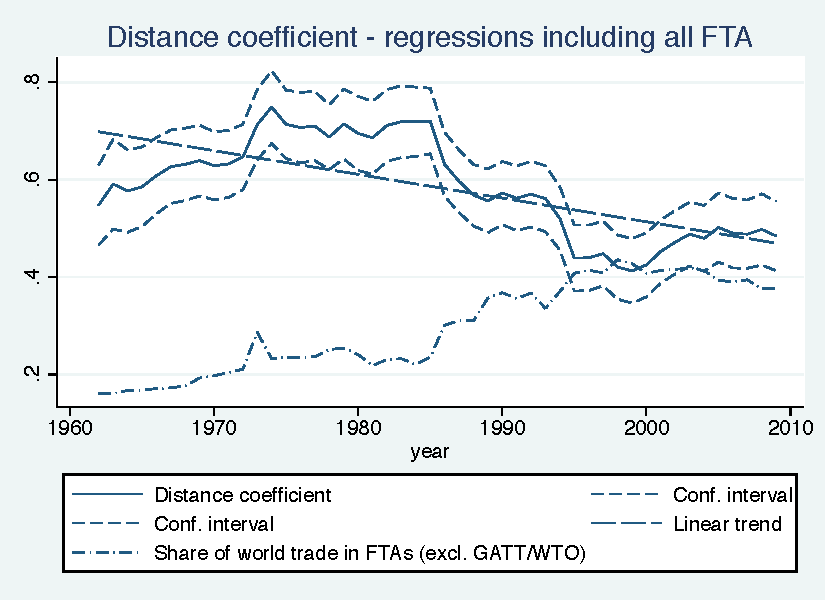
\includegraphics[trim = 0mm 0mm 0mm 9.5mm, clip,height=2.5in]{graph6.pdf}}
%\end{center}
%\end{figure}
%As shown in Figure 
\ref{fig:ftas}, controlling for countries' participation into free trade agreements solves the distance puzzle.
However, this effect is mechanical.
Indeed, Figure 
\ref{fig:ftas} shows that in-FTA trade increased from less than 20\% to approximately 40\% of total trade from 1962 to 2009, and Figure 
\ref{fig:ftascontig} shows that over the same period the share of intra-FTA trade among nearby (less than 2000 km) countries increased from 38\% to 79\% in 2009.\footnote{Trade at less than 2000 km corresponds to the first decile of the distance distribution of trade in 1962-2009.} This means that including controls for FTA membership amounts to adding a growing number of proximity controls in the regression.
This reduces the sensitivity of trade flows to distance.

%A further argument for caution in interpreting results with FTA controls is the probable endogeneity of FTAs for which we do not correct in the estimation.
In this respect, \cite{Bosquet2015} show that the distance coefficient evolves in the same way when they do not control for FTAs (Figure 
9 in their paper) and when they control for FTAs correcting for endogeneity (Figure 
11 in their paper).
%\begin{figure}[H]
%\caption{FTAs as proximity controls (full sample) \label{fig:ftascontig}}
%\begin{center}
%\setlength{\fboxrule}{1pt} %makes border lines thick
%\setlength{\fboxsep}{.1in} %increases distance to border
%\fbox{\includegraphics[trim = 0mm 0mm 0mm 9.5mm, lip,height=3.2in]{graph_ftas_contig.png}}
%\end{center}
%\end{figure}
%Controlling separately and jointly for sample and composition effects does not change the magnitude of the distance puzzle.
On the other hand, controlling for FTAs eliminates the distance puzzle.
As argued, the explanation of the distance puzzle through FTAs is not satisfactory because it amounts to adding a growing number of proximity controls in the regression and because FTAs are endogenous to trade intensity.
We conclude that the distance puzzle is a robust feature of the data, and that the traditional approach is little informative of the driving forces behind the increased sensitivity of trade flows to distance.
 
\fi

%SUMMARY: RECAP TABLE UPDATED for 1962-2013 *no FTA*
\subsection{Summing up: the robustness of the distance puzzle}\label{part1recap}
\begin{table}[h!]
\caption{Evolution of $\delta_t$: sample, composition and FTA effects \label{tab:part1recap}}
\begin{center}
\begin{tabular}{|l|c|c|c||c|c|c|}
\hline
        & \multicolumn{3}{|c||} {FULL} & \multicolumn{3}{|c|} {STABLE} \\
\hline
        & {rate (\%)} & {R-sq} & {total change} & {rate (\%)} & {R-sq} & {total change} \\
\hline
Baseline  & $.09^{*}$ & $.07$ & $1.045$ & $.33^{***}$ & $.49$     & $1.182$ \\
\hline
World bundle & $.26^{***}$ & $.53$ & $1.145$ & $.33^{***}$ & $.68$ & $1.184$ \\
\hline
Country bundle & $.40^{***}$ & $.87$ & $1.227$ & $.54^{***}$ & $.77$ &  $1.314$ \\
\hline
\multicolumn{7}{|l|}{\begin{footnotesize} Note: Estimated annualized growth rates reported in col.2 and col.5 are obtained as a geometric fit on the\end{footnotesize}} \\
 \multicolumn{7}{|l|}{\begin{footnotesize} basis of annual point estimates of the distance coefficient in 1962-2013.
Col.3 and col.6 report the share \end{footnotesize}} \\
 \multicolumn{7}{|l|}{\begin{footnotesize} of time variation in the point estimate explained with the annualized growth rate.

 \end{footnotesize}} \\
 \hline
\end{tabular}  
\end{center}
\end{table}
%Remember that corrfta computed in full sample on basis of distfix70, but results very similar for distfix63
Table \ref{tab:part1recap} summarizes our findings.
The distance puzzle is magnified in the sample of stable pairs and robust to fixing the product composition of world trade.
Hence, the non-decreasing distance elasticity of trade is likely to be a structural outcome rather than an artefact of composition effects.
\if 0 
Furthermore, trade intensification through FTA formation does not help to explain the distance puzzle.\footnote{Results are mitigated in the stable sample where the corrected FTA specification performs poorly.}
The process of regional integration appears to have been working through the extensive margin, e.g.
through the increasing geographic scope of FTAs and their increasing coverage of short-distance trade rather than through the intensification of within-FTA trade.
\fi
These results motivate our focus on structural heterogeneity as a possible alternative explanation of the non-decreasing distance elasticity.


\clearpage

\section{ Interpreting the distance coefficient}
In the three canonical microfoundations of the gravity model, the distance coefficient $\delta $ is the product of two elasticities: the elasticity of trade costs to distance $ \rho $ and the elasticity of trade flows to trade costs $ \epsilon $.
The question addressed in this paper is very simple.
Have trade flows become more sensitive to trade costs (increasing $ |\epsilon| $), or have trade costs become more sensitive to distance (increasing $\rho$)? 
The three main microfoundations of the gravity model of trade give structurally different interpretations to $ \epsilon $ but not to $ \rho $. 
In this section, we briefly discuss the interpretation of the structural parameter $ \epsilon $ in each model and review the evidence on its evolution. 
%Assuming that the magnitude of $ \rho $ is determined by the structural features of the transport sector (global trade system), and as such invariant to the microfoundation of the gravity model, the evolution of the trade elasticity $ |\epsilon| $ is also expected to be model-independent.  
We then provide details on the procedure used in section {\hyperref[ref-003]{3}} to pin down the evolution of $ \epsilon $ in one of these canonical microfoundations, namely the Armington framework. 

\subsection{What does the trade elasticity $ \epsilon $ actually measure? }

In \cite{Eaton2002} the heterogeneity dimension captured by the trade elasticity $ \epsilon $ is intersectoral.
Consumers maximize a CES utility function defined at the intersectoral level by shopping around the world for the cheapest supplier of each sectoral good. 
$|\epsilon|$  is decreasing in the degree of intersectoral productivity dispersion.
If sectoral productivity draws become more similar, trade flows become more responsive to trade costs.

In the \cite{Melitz2003}-\cite{Chaney2008} framework the heterogeneity dimension captured by the trade elasticity $ \epsilon $ is intrasectoral.
Consumers value firm-specific varieties of goods which they acquire in monopolistic competition markets.
$ |\epsilon| $ is decreasing in the degree of intrasectoral productivity dispersion.
If firm productivity draws become more similar, trade flows become more responsive to trade costs.

In \cite{Anderson2003} there is no heterogeneity in productive efficiency, and
%The production process in each country and sector is constant returns to scale.
product markets in each country are competitive.
So production costs are equalized across goods within a country.
The heterogeneity dimension comes from the assumption that consumers perceive goods of different national origin as intrinsically imperfect substitutes.
Each country is specialized in production of country-specific goods which on aggregate give a country-specific composite good.
$|\epsilon|$ is increasing in the perceived substitutability of goods of different origin. 
The trade elasticity $\epsilon$ equals $1-\sigma$, where $\sigma$ denotes the lower tier Armington elasticity of substitution.\footnote{In classical work on the price sensitivity of import demand, the upper-tier elasticity measures substitutability of domestic products and an aggregate import good.
The lower-tier one measures substitutability between importers of a given good.
See \cite{Sato1967}, \cite{Reinert1991}, \cite{Saito2004}, and \cite{Feenstra2018}.} 

\subsection{What do we know about the evolution of the trade elasticity?}

Neither of these models incorporates a theoretical mechanism that would explain a change in the trade elasticity.
A shock to consumer preferences or to the shape parameter of the productivity distribution would be required. This implicit assumption of stability in the structural parameters, together with data availability constraints, explain why there is only scant empirical evidence on the evolution of sectoral or aggregate trade elasticities in either model. 

There is no direct evidence on the evolution of productivity dispersion across firms over 1960-2010.\footnote{There is some evidence of an increasing productivity dispersion in the set of surviving firms over 2000-2015, but the latter may be a consequence of more integrated global markets (\cite{DiGiovanni2011}).}
Different theoretically grounded methods have been used to estimate the intersectoral productivity dispersion parameter, i.e. the trade elasticity in the Ricardian framework, but only in a specific year.\footnote{\cite{Eaton2002}; \cite{Simonovska2014}; \cite{Costinot2012a}; \cite{Caliendo2015}.}  To our knowledge, \cite{Levchenko2016} is the only paper that looks into  the evolution of intersectoral productivity dispersion. They find evidence of within-country convergence in sectoral knowledge stocks over 1960-2010.
%As there is less heterogeneity in producer efficiency across the set of goods comparative advantage exerts a weaker force against trade resistance imposed by trade barriers.
Reduced dispersion in sectoral productivity draws would translate into an increasing $|\epsilon|$ in the Ricardian framework.

Evidence on the evolution of lower-tier Armington elasticities of substitution measured on aggregate data is scarce.
For France, \cite{Welsch2006} provides estimates of aggregate lower-tier Armington elasticities since the 1970s.
He finds that among exporters to the French market the elasticity peaked in the 1970s, and progressively decreased in the 1990s.
\cite{Broda2006} provide evidence on the evolution of Armington lower-tier elasticities between 1972-1988 and 1990-2001 for American imports.
They find that the mean and median elasticities decreased for all types of goods at all levels of product disaggregation, i.e.
at the 10-digit, 5-digit, and 3-digit levels.
Lower perceived substitutability of products of different national origin would translate into a decreasing trade elasticity in the Armington framework,  deepening the distance puzzle. 
%INCLUDE DISCUSSION OF WHY BW approach may be undesirable: number of flows increases; requires reduction in substitutability to accomodate increasing variety

\subsection{ A method to measure the trade elasticity in the Armington framework}

To tease out the aggregate trade elasticity in the Armington framework that can contribute to solving the aggregate distance puzzle, it is necessary to  constraint the trade elasticity to be invariant across sectoral goods and destination markets.To the best of our knowledge, no paper has as yet provided evidence on the evolution of the Armington elasticity for aggregate bilateral trade in that context. \footnote{\cite{Head2013} put forward that the heterogeneity in the trade elasticity across trading pairs and changes in trade participation led to an increase in the aggregate trade elasticity. Our focus is on an alternative - and possibly complementary - mechanism, namely an increase in the perceived similarity of products of different origin.} 

We focus on the Armington framework for two main reasons. 
First, as we want to measure the trade elasticity from 1963 for all countries involved in world trade, we operate in a data-poor environment. 
We believe that the biases entailed by this lack of information do not make the exercise worthless because we are interested in the evolution of the parameter rather than in its exact value.
We do not have sufficient information on disaggregated bilateral tariffs to carry out the estimation in a model-independent way.\footnote{See \cite{Head2001} and \cite{Caliendo2015} for the methodology.
\cite{Caliendo2015a} build a comprehensive dataset on bilateral tariffs that covers 1990-2010.
A novel model-independent approach is proposed in \cite{Allen2019} that only requires data on income and gross output of each country.
Although in principle feasible, this approach also requires constructing a set of instruments, the hypothetical values of income and gross output, and it delivers an estimate of the trade elasticity that is relatively imprecise.} 
Nor do we have information on the distribution of domestic prices or disaggregated data on domestic production needed to estimate the trade elasticity in the Ricardian framework.
The available trade data is amenable to the estimation of the Armington elasticity only in cross-section.
 
Second, as put forward in recent work, the disappearance of the demand parameter from the trade elasticity is a consequence of opting for an unbounded Pareto in modelling the firm productivity distribution in the Meltiz framework. Under less restrictive assumptions, the trade elasticity is a function of 2 or more parameters, and in particular combinations of demand and supply side parameters.\footnote{See \cite{Costinot2014}, \cite{Bas2017}, \cite{Feenstra2018}, \cite{Feenstra2018a}.} The coefficient is increasing in the magnitude of the Armington elasticity.

Measuring the Armington elasticity is a perennial issue in the trade literature. 
\cite{Feenstra2018} discuss the difficulties involved and implement a state-of-the art method to estimate both the upper-tier import demand elasticity (between the domestic good and the imported composite good) and the lower-tier Armington elasticity (between different foreign goods).
\footnote{The seminal paper using time variation in prices and quantities across a set of destination markets to pin down the lower-tier Armington elasticity for a specific product is \cite{Feenstra1994}. For subsequent refinements see \cite{Broda2006b}, \cite{Imbs2015}, and \cite{Soderbery2015}.}

We depart from this literature and suggest a cruder estimation method in part because we operate in a data-poor environment but also for more fundamental reasons.
First, Feenstra's method and its developments rely on the assumption that the elasticity parameter remains constant through time, whereas our research question implies that the parameter can vary from year to year.
Second, Feenstra's elasticity parameter determines short-run, marginal, longitudinal effects whereas we are interested in the elasticity parameter which determines long-run, equilibrium, cross-section outcomes.
While we admit that in most tractable theoretical settings these parameters would be the same, it is useful to bring this question to the data.
%It is not immediate that they are the same in the data.

The UN COMTRADE database gives information on bilateral trade flows and cif unit values at the SITC 4-digit level since 1962 for the majority of countries.
These data are sufficient to estimate the trade elasticity in the Armington framework.
The perceived substitutability of imported sectoral goods can be estimated on the basis of the distribution of prices and of market shares in each market and each destination.
%If we have importer-specific prices in destination markets and importer-specific market share, we should be able to observe some statistical regularities.

The basic intuition of the method we use starts from the demand equation for an exporter-specific sectoral good in the one-good Armington framework (assuming a CES utility function):
\[{{X}_{ij}}={{\left( \frac{{{P}_{ij}}}{{{P}_{j}}} \right)}^{1-\sigma}}{{Y}_{j}}\]
where ${X}_{ij}$ is the cif value of the exports from $i$ to $j$, ${{P}_{ij}}$ is the cif price of the good shipped from $i$ to $j$ and ${{P}_{j}}$ is the price index in the destination and ${{Y}_{j}}$ total import demand in the destination.
The exponent $\left( 1-\sigma \right)$ captures the substitutability of country-composite goods across frameworks.
It is also the aggregate trade elasticity $\epsilon $ in the Armington framework.
Briging this equation to the data is difficult, however, as we do not observe aggregate prices, but unit values at the SITC 4-digit category level.
Still, the distance puzzle concerns an elasticity estimated on aggregate trade data.
As shown by \cite{Imbs2015} this parameter cannot generally be mimicked by a theoretically grounded weighted average of sector-specific trade elasticities.
Hence, we need an estimation procedure that works directly with aggregate data.

Define aggregate imports from source country $i$ to destination country $j$  as the sum of imports from each sector $k$ where a sector corresponds to a SITC 4-digit category: ${{X}_{ij}}=\sum\limits_{k}{{{X}_{k,ij}}}$.
Given CES utility at the intersectoral level, sectoral demand in country  in sector  for imported goods is given by: 
\[\begin{array}{*{35}{l}}
   {{Y}_{k,j}} & = & {{\left( \frac{{{P}_{k,j}}}{{{\beta }_{k}}{{P}_{j}}} \right)}^{1-\sigma }}{{Y}_{j}}  \\
\end{array}\]
Where ${{P}_{k,j}}$ and ${{P}_{j}}$ are price indexes, ${{\beta }_{k}}>0$ is a sector-specific preference parameter, ${{Y}_{j}}$ is total demand for imported goods, $\sigma >1$ is the elasticity of substitution between sectors.

 Assume each country exports a specific national variety.
Preferences within each sector $k$ between national varieties are assumed well represented by a CES utility function with the same $\sigma $ parameter as the intersectoral CES utility function.
Intrasectoral demand for varieties exported by $i$ in $j$ in sector $k$ is: 
\[\begin{array}{*{35}{l}}
   {{X}_{k,ij}} & = & {{\left( \frac{{{p}_{k,ij}}}{{{\gamma }_{i}}{{P}_{k,j}}} \right)}^{1-\sigma }}{{Y}_{k,j}}  \\
\end{array}\]
Where ${{\gamma }_{i}}>0$ is a origin-country-specific preference parameter and ${{P}_{k,j}}$ is the CES price index:
\[\begin{array}{*{35}{l}}
   {{P}_{k,j}} & = & {{\left[ \sum\limits_{i\ne j}{{{\left( \frac{{{p}_{k,ij}}}{{{\gamma }_{i}}} \right)}^{1-\sigma }}} \right]}^{1/(1-\sigma )}}  \\
\end{array}\]
  Defining $\frac{{{Y}_{k,j}}}{{{Y}_{j}}}={{\omega }_{k,j}}$, we get: 
\[\begin{array}{*{35}{l}}
   \frac{{{X}_{k,ij}}}{{{Y}_{j}}} & = & {{\omega }_{k,j}}{{\left( \frac{{{p}_{k,ij}}}{{{\gamma }_{i}}{{P}_{k,j}}} \right)}^{1-\sigma }}  \\
\end{array}\]
 Summing over all SITC 4-digit sectors: 
\[\begin{array}{*{35}{l}}
   \sum\limits_{k=1}^{K}{\frac{{{X}_{k,ij}}}{{{Y}_{j}}}}=\frac{{{X}_{ij}}}{{{Y}_{j}}} & = & \gamma _{i}^{\sigma -1}\sum\limits_{k=1}^{K}{{{\omega }_{k,j}}}{{\left[ \frac{{{p}_{k,ij}}}{{{P}_{k,j}}} \right]}^{1-\sigma }}  \\
\end{array}\]
Changing notation to $\kappa_i=\gamma_i^{\sigma-1}$, the market share equation for aggregate bilateral trade in a destination market is defined as a function of the weighted average of sectoral relative prices: 

\begin{eqnarray}
   \frac{{X}_{ij}}{Y_j} & = & {{\kappa }_{i}}\sum\limits_{k=1}^{K}{{{\omega }_{k,j}}}\frac{p_{k,ij}^{1-\sigma }}{\sum\limits_{l\ne j}{{{\kappa }_{l}}}p_{k,lj}^{1-\sigma }}  
\end{eqnarray}

As this is a market share, it is reasonable to assume that the errors are multiplicative.
Measurement errors on a market share of 1\% cannot be the same in percentage points as measurement errors on a market share of 10\%.
We have to fit the following model to the data:
\begin{eqnarray}
   \frac{{{X}_{ij}}}{{{Y}_{j}}} & = & {{\kappa }_{i}}\sum\limits_{k=1}^{K}{{{\omega }_{k,j}}}\frac{p_{k,ij}^{1-\sigma }}{\sum\limits_{l\ne j}{{{\kappa }_{l}}}p_{k,lj}^{1-\sigma }}.{{e}^{{{\varepsilon }_{i,j}}}}
  \end{eqnarray}

Notice that we only have non-zero observations, as ${{p}_{k,ij}}$ is only observed when there is a trade flow.
We take logs to transform the errors into additive ones and estimate the following equation for each year with a non-linear least square procedure in STATA:
\begin{eqnarray}
   \ln \left( \frac{{{X}_{ij}}}{{{Y}_{j}}} \right) & = & \ln {{\kappa }_{i}} +\ln \left( \sum\limits_{k=1}^{K}{\frac{{{Y}_{k,j}}}{{{Y}_{j}}}.}\frac{p_{k,ij}^{1-\sigma }}{\sum\limits_{l\ne j}{{{\kappa }_{l}}}p_{k,lj}^{1-\sigma }} \right) +{{\varepsilon }_{i,j}}
   \label{eqn:nlestimation}
   \end{eqnarray}
   
This approach yields annual estimates of ${{\kappa }_{i}}$ and $\sigma $.\footnote{Because of the way the procedure \textit{nl} works in STATA, instead of minimizing $\sum\limits_{i,j}{{{\left( {{\varepsilon }_{ij}} \right)}^{2}}}$, it minimizes $\sum\limits_{i,j}{{{n}_{ij}}{{\left( {{\varepsilon }_{ij}} \right)}^{2}}}$ where ${{n}_{ij}}$ is the number of 4-digit sectors in which imports from $i$ to $j$ are recorded.
As a result, we have to weight each observation in the regression by $1/{{n}_{ij}}\ $ to make its results comparable to those in part one.
}


\section{ Evolution of the Armington trade elasticity from 1963 to 2013}

In this section we first discuss the results of the baseline estimation of equation (\ref{eqn:nlestimation}). 
We then carry out a series of robustness checks to deal with missing unit values, zero trade flows, low data quality and endogeneity.
We conclude with an interpretation of the distance puzzle through the lens of the Armington framework by decomposing the  in the distance coefficient into the part attributable to the change in the trade elasticity and the part attributable to the change of the elasticity of trade costs to distance $ \rho $. 
%Under the assumption of model independence, this decomposition of the movement in the distance coefficient across the two elasticities is expected to carry over to an alternative microfoundation of the gravity model.

\subsection{Results}\label{subsec:baseline}

The baseline estimation of equation (\ref{eqn:nlestimation}) is carried out on annual cross-sections of the UN COMTRADE dataset.
We work with the data at the 4-digit level, and we consider as separate goods trade flows with quantities measured in different units (kg,l,items). 
We therefore refer to the level of disaggregation as $4'$-digit.
We drop bilateral trade flows with missing information on quantity as well as trade flows and unit values with negative or zero values.
We drop information on exporters whose market share is smaller than .1\% of global trade. 
We drop bilateral trade flows whenever the associated unit value is in the top or bottom 5 percentiles of the unit value distribution in this product and destination market at the $4'$-digit level.
We also drop trade flows whenever the associated unit value is more than two orders of magnitude smaller or bigger than the median unit value in the product and destination market.

%{\hyperref[ref-005]{Figure 5}} 
Figure \ref{fig:baseline} presents the results.
The absolute value of the estimated trade elasticity $|1-\sigma|$ has increased by 22\% from 1962 to 2013.
This corresponds to an annual increase of .4\% per year.\footnote{The estimated annualized growth rate is significant at 1\% level, the 95\% confidence interval is between 0.15\% and 0.63\% (not taking into account though the uncertainty around yearly estimates).}
%According the preceding discussion, this is a lower bound on the increase in the underlying substituability parameter.

%\textbf{Figure 5: Estimated $(1-\sigma)$}
%\includegraphics[width=1\textwidth]%{1ere_regression_3e_partie.eps} \label{fig_baseline}
\begin{figure}[H]
\caption{Estimated $(1-\sigma)$, baseline\label{fig:baseline}}
\begin{center}
\setlength{\fboxrule}{1pt} %makes border lines thick
\setlength{\fboxsep}{.1in} %increases distance to border
\fbox{\includegraphics[trim = 0mm 0mm 0mm 0mm, clip, height=2.7in]{"1ere regression 3e partie_baseline".pdf}}
\end{center}
\end{figure}

The magnitude of the estimated trade elasticity (in absolute value) is in the low range, i.e. $|1-\sigma|=\left\{.4,.5\right\}$. Working with US data, \cite{Feenstra2018} obtain a point estimate in the $\left\{0.5,3\right\}$ range, depending on the estimator used, while \cite{Imbs2015} obtain a point estimate of $1-\sigma=-2$.\footnote{The time variation in market shares and prices across US trade partners is used in these papers while we work off market share and price variation in a single cross-section.}
%1992-2007 used in Feenstra2018; 1996-2004 used in Imbs and Mejean

\subsection{Robustness checks}
%phrase a mettre en lien avec la discussion des robustness checks (effets de composition)
%The magnitude of the trade elasticity measured on aggregate trade data could have evolved over 1962-2013 without any shock to the underlying heterogeneity, in particular through changes in the range of traded goods or because of time-sensitive aggregation issues linked to estimating a single parameter across sectors. 
\subsubsection{ The incidence of missing unit values}
The COMTRADE dataset does not provide quantities for all non-zero trade flows.
It is not possible to compute unit values in these cases.
Figure \ref{fig:missing_uv}, \textit{4'-digit} indicates how often that happens from 1962 to 2013.
The problem arises for a small share of the total trade value (never more than 25\%).
In the baseline estimation, we have simply dropped these observations. As a robustness check, it is possible to approximate missing unit values by unit values from similar products using a stepwise price imputation procedure.


\begin{figure}[H]
	\caption{Trade with missing unit values}
	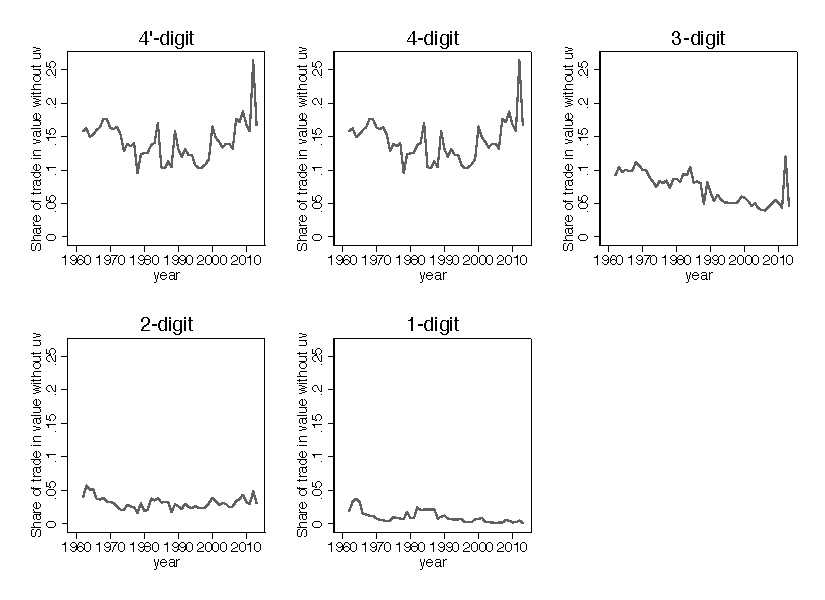
\includegraphics[width=1\textwidth]{Graph_missing_uv.pdf}
	\label{fig:missing_uv}
	\caption*{The way to read this graph is : In 1962, 10\% of trade is in a 3-digit bilateral trade category that does not mention at least one unit value}
\end{figure}




%To deal with missing uv, we impute prices 
%Guillaume DaudinGD2016-04-20T14:47:00Z Guillaume DaudinGD Guillaume DaudinGD Guillaume Daudin Guillaume Daudin GD GD 2016-04-20T14:47:00Z 2016-04-20T14:47:00Z Enlev\'{e} :~The weighted average price at a higher aggregation level for this sector and source will be used for the unobserved price.
%An alternative procedure consists in imputing the relative price observed at the same disaggregation level for another source with a similar market share in this sector and destination.
%Results are not sensitive to the procedure used.
%Enlev\'{e} :~The weighted average price at a higher aggregation level for this sector and source will be used for the unobserved price.
%An alternative procedure consists in imputing the relative price observed at the same disaggregation level for another source with a similar market share in this sector and destination.
%Results are not sensitive to the procedure used.
%.

In this procedure, whenever possible, we first compute unit values at the highest disaggregation level for each product and quantity unit provided by the source (the \textit{4'-digit} level).
When this is missing, we compute de trade-weighted mean relative unit value at the 4-digit level for this importer and use it to impute an absolute unit value at the \textit{4'-digit} level.

%We then proceed level by level for aggregation: the relative price of the composite sectoral good of the source is constructed at the 4-digit level using the weighted average relative price observed at the 4'-digit level, with destination-specific weights for each variety of the 4'-digit good the source is active in. 
%Guillaume DaudinGD2016-04-20T14:47:00Z Guillaume DaudinGD Guillaume DaudinGD Guillaume Daudin Guillaume Daudin GD GD 2016-04-20T14:47:00Z 2016-04-20T14:47:00Z Given relative prices constructed at the 4-digit level, destination-specific weights are used to aggregate these up to the 3-digit level, and so on until the relative price for the composite good is constructed using relative prices at the 1-digit level.
%Given relative prices constructed at the 4-digit level, destination-specific weights are used to aggregate these up to the 3-digit level, and so on until the relative price for the composite good is constructed using relative prices at the 1-digit level.
%.
If no relative unit value is available at the 4-digit level, we move at the 3-digit level, etc.
As Figure \ref{fig:missing_uv} shows, that procedure allows to reduce considerably the share of trade without unit values.
This procedure is justified if one assumes that missing destination-specific relative unit values at the 4'-digit can be approximated by the mean observed destination-specific relative price among the corresponding 4-digit group, or 3-digit...

Figure \ref{fig:reg_prix_calc} shows that our result hold to the use of imputed prices. The yearly increase of the absolute value of the estimated $|1-\sigma|$ is 0.6\% instead of 0.4\%, for a total increase of 35\% over the whole period.

\begin{figure}[H]
	\caption{Estimated $(1-\sigma)$ , with imputed prices}
	\includegraphics[width=1\textwidth]{"1ere regression 3e partie_prix_calc".pdf}
	\label{fig:reg_prix_calc}
\end{figure}



\subsubsection{ Zero trade flows}
A second difficulty arises when both quantity and value data are missing.
Zero trade flows (ztf) are a prevalent feature of the data even though under model assumptions some trade should be observed in every sector \textit{k} between all pairs \textit{ij}.
The share of observed SITC 4-digit flows relatively to the total number of potential SITC 4-digit bilateral trade flows increases from c. 3.5\% to c. 9\% between 1962 and 2013 (see Figure \ref{fig:share_of_ztf}).
The existence of zero trade flows can be reconcilied with our theoretical framework by assuming that the underlying trade flows are strictly positive but so small that they do not pass the threshold applied by the data collecting authorities (in UN COMTRADE this threshold corresponds to 1000 USD).
Still, the implied biais (if any) in our estimate is not clear. 

To test the robustness of our results to this issue, we restrict the estimation to the "superbalanced" sample (see note \ref{fnsuperbalanced}). 
Figure \ref{fig:share_of_ztf} shows that the share of zero trade flows is smaller in the superblanced sample.
The evolution of non-zero trade flows is similar in both samples.
In both cases, it is multiplied by approximately 2.5.
One would thus expect that any biais linked to the presence of zero trade flows would attenuated by the study of the superblalanced sample.
Figure \ref{fig:reg_superbal} shows that the increase in the absolute value of estimated $|1-\sigma|$ is faster: 1\% a year instead of 0.4\% a year, for a predicted total increase of 69\% over the whole period. That suggests that, in itself, the large prevalence of zero trade flows does not lead to an over-estimation of the increase of $|1-\sigma|$.

\begin{figure} [H]
	\caption{Share of zero trade flows}
	\includegraphics[width=1\textwidth]{"graph_ztf".pdf}
	\label{fig:share_of_ztf}
\end{figure}


\begin{figure} [H]
	\caption{Estimated $(1-\sigma)$ , superbalanced sample}
	\includegraphics[width=1\textwidth]{"1ere regression 3e partie_superbal".pdf}
	\label{fig:reg_superbal}
\end{figure}

%The consequences for our estimation procedure depend on the reason why such flow does not pass the threshold.
%Using the notations of equation {\ref{eqn:nlestimation}), that can be either because because $\kappa_i$ is small or because $p_{k,ij}$ is very large.
%	
%If this happens because $p_{k,ij}$ is large, $\frac{p_{k,ij}^{1-\sigma }}{\sum\limits_{l\ne j}{{{\kappa }_{l}}}p_{k,lj}^{1-\sigma }}$ will be small and hence the overestimation of the relative price of goods from country $i$, $\sum\limits_{k=1}^{K}{\frac{{{Y}_{k,j}}}{{{Y}_{j}}}.}\frac{p_{k,ij}^{1-\sigma }}{\sum\limits_{l\ne j}{{{\kappa }_{l}}}p_{k,lj}^{1-\sigma }}$ will be small as well.
%This is not too much of a threat to the validity of our estimation procudure.
%
%If this happens because $\kappa_i$ is small, as might be possible for small exporters, this means that $X_{ij}$ will be systematically under-estimated. If small exporters have systematically higher prices than large exporters, that means that the effect of prices on market share will be systematically over-estimated.

%
%Such flows, if recorded, would not substantially modify the distribution of observed market shares in the destination (the left hand side of equation {\ref{eqn:nlestimation}) because they are an order of magnitude smaller than observed trade.
%	Still, we have to make some assumption about their price to be able the effect of price on market shares.
%	
%	
%	This is only possible when zero trade flows are present in an existing bilateral relation.
%	In this case, we use the same stepwise price imputation for zero trade flows as in the case of missing unit values.
%	This is problematic because statistically unobserved trade values logically correspond to a higher cif price than the maximum observed price in the destination across all sources and sectors while by construction we postulate that unobserved relative prices in ztf sectors are equal to a weighted average relative price across sectors in which bilateral trade is observed.
%	\footnote{An alternative method consists in imputing unobserved relative prices with some arbitrary price above the maximum observed in the destination.
%		As ztf constitute 91-96\% of all 4-digit trade flows, this method is problematic because results are driven by imputed rather than observed prices.
%	}
%	
%	This assumption would not bias our estimate if the underestimation factor were constant across exporters.
%	This scalar would cancel out across sources, and the estimated substitutability parameter would correspond to the true parameter.
%	
%	
%	
%	{\hyperref[ref-005]{Table 2}} shows it is not the case.
%	The share of ztf is strongly decreasing in market share, i.e.
%	the underestimation factor is larger for small exporters (though they already have higher prices).
%	As a result, for a given observed distribution of market shares, the underlying dispersion in relative prices of the composite good is greater than the observed dispersion in relative prices.
%	This means that the estimated parameter $(1-\tilde{\sigma })$ overestimates the true substitutability parameter $(1-\sigma)$.
%	
%	{\hyperref[ref-005]{Table 2}} shows that the reduction in the share of ztf proceeds at quicker pace in 1962-2013 for small exporters: the coefficient for the interaction term for the market share and year is significant and positive.
%	{\hyperref[ref-006]{Table 3}} presents the predicted share of ztf for four types of exporters in 1962 and 2013.
%	For a  small exporter with .01\% market share, the initial share of ztf is predicted to be .99, and it is reduced to .86 by 2009, i.e.
%	a 13 percentage point decrease.
%	Consider a large exporter, with a .6\% market share: its share of ztf is reduced from .86 to .76, a 10 percentage point decrease.
%	As the gap between the share of ztf for big and small exporters is reduced overtime, the overestimation bias of $(1-\tilde{\sigma })$ is progressively reduced.
%	
%	%Guillaume DaudinGD2016-04-20T14:47:00Z Guillaume DaudinGD Guillaume DaudinGD Guillaume Daudin Guillaume Daudin GD GD 2016-04-20T14:47:00Z 2016-04-20T14:47:00Z noteLA: J'enleve la phrase qui suit parce que ce qui compte c'est l'\'{e}cart entre les deux et non pas le fait que les prix soient sous-estim\'{e}s pour les petits.
%	%Hence, the overestimation of the underling ${\sigma}$ by the estimated substitutability parameter ${\sigma}$ because of the under-estimation of small exporters' prices declines over time.' noteLA: J'enleve la phrase qui suit parce que ce qui compte c'est l'\'{e}cart entre les deux et non pas le fait que les prix soient sous-estim\'{e}s pour les petits.
%	%`Hence, the overestimation of the underling ${\sigma}$ by the estimated substitutability parameter ${\sigma}$ because of the under-estimation of small exporters' prices declines over time.' noteLA: J'enleve la phrase qui suit parce que ce qui compte c'est l'\'{e}cart entre les deux et non pas le fait que les prix soient sous-estim\'{e}s pour les petits.
%	%`Hence, the overestimation of the underling ${\sigma}$ by the estimated substitutability parameter ${\sigma}$ because of the under-estimation of small exporters' prices declines over time.' 
%	
%	
%	\begin{table}
%		\caption{ \label{ref-005} Proportion of zero trade flows as a function of market share (4' digits)}
%		\begin{tabular}{lcccc}
\multicolumn{5}{c}{Proportion of zeros as a function of market share} \\ \hline
 & (1) & (2) & (3) & (4) \\
VARIABLES & propor\_ssuv\_5 & propor\_ssuv\_5 & propor\_ssuv\_5 & propor\_ssuv\_5 \\ \hline
 &  &  &  &  \\
ln\_ms & -0.0330*** & -0.1261*** & -0.0350*** & -0.1542*** \\
 & (0.0001) & (0.0098) & (0.0001) & (0.010) \\
year & -0.0026*** & -0.0022*** & -0.0030*** & -0.0025*** \\
 & (0.0000) & (0.0001) & (0.0000) & (0.000) \\
interaction &  & 0.0000*** &  & 0.0001*** \\
 &  & (0.0000) &  & (0.000) \\
Constant & 4.8436*** & 4.0417*** & 5.6383*** & 4.6135*** \\
 & (0.0244) & (0.1007) & (0.0270) & (0.098) \\
 &  &  &  &  \\
 Observations & 749,686 & 749,686 & 749,686 & 749,686 \\ \hline
\multicolumn{5}{c}{ Robust standard errors in parentheses} \\
\multicolumn{5}{c}{ *** p$<$0.01, ** p$<$0.05, * p$<$0.1} \\
\multicolumn{5}{c}{ The proportion of zeros is computed at the SITC 5-digit level.} \\
\end{tabular}

%		
%	\end{table}
%	
%	
%	%\textbf{Table 3: Predicted share of ztf for exporters with different market share, 4'-digit level \label{ref-006}}
%	
%	\begin{table}[tbp] \centering
\newcolumntype{C}{>{\centering\arraybackslash}X}

\caption{Predicted share of ztf for exporters with different market share, 4'-digit level}
\begin{tabularx}{\textwidth}{lCCCC}

\toprule
{}&{At mean}&{At meand and 2sd}&{At ln(0.01)}&{At ln(0.1)} \tabularnewline
\midrule\addlinespace[1.5ex]
1962&.92&.75&.84&.78 \tabularnewline
1987&.89&.71&.79&.73 \tabularnewline
2013&.88&.67&.74&.69 \tabularnewline
\bottomrule \addlinespace[1.5ex]

\end{tabularx}
\begin{flushleft}
\footnotesize Notes: This is based on the regression in column (2)
\end{flushleft}
\end{table}
\label{ref-006}
%	
%	
%	
%	%Columns (1) and (4) correspond to the mean and to 2 st.
%	%deviations above the mean in the distribution of log market share.
%	%Columns (2) and (3) correspond to the mean and to 2 st.
%	%deviations above the mean in the distribution of market share.
%	
%	
%	Thus, the hypothesis we make on unobserved sectoral prices in ztf sectors will not always impede interpreting the evolution of the underlying substitutability parameter.
%	In particular, because the overestimation bias is reduced overtime, if it is found that the estimated parameter increases in absolute value, this evolution necessarily provides a lower bound on the increase in the underlying substitutability parameter.
	
\subsubsection{Changing the dataset\label{baci}}
The UN COMTRADE dataset mostly simply brings together trade reported by individual countries.
For example, it does not try to reconcile contradictory declarations for mirror flows.
It is possible to increase the quality of the data by conducting an harmonization procedure.
That has been don by the CEPII with the BACI dataset that reports bilateral trade data at the HS-1992 6-digit disaggregation level for 1995-2016 (Gaulier et Zignago 2010).
As a result, BACI includes much better-quality unit values while substantially reducing the number of observations with lacking unit value.
At the 6-digit level, less than 7\% of total reported trade in BACI has missing unit values.

%The accuracy of the relative prices of country-composite goods constructed with this dataset is improved because the harmonization procedure applied by (Gaulier et Zignago 2010) in constructing BACI yields much better-quality unit values while substantially reducing the number of observations with lacking unit value.
%As a result, at the 6-digit level, less than 7\% of total reported trade in BACI has missing unit values.
%This is reduced to 1-3\% of total trade when the data is aggregated to the 4-digit level, as opposed to more than 10\% in the raw COMTRADE data we originally used.
%Another advantage is that the share of ztf in BACI is stable in 1995-2009 as opposed to relatively strong fluctuations in the share of ztf overtime in our original dataset.
The disadvantage of BACI is that it covers only a relatively short period compared to the years over which the distance puzzle exists.
Still, it is interesting to see if our estimated evolution of $|1-\sigma|$ is robust to the use of this better dataset.
Obviously, we do not expect to reproduce exactly our baseline results because the trade classification and its level of aggregation are different
Figure \ref{fig:reg_Baci} shows that our results hold: the absolute value of $|1-\sigma|$ increases from 1995 to 2016.
The speed of increase is faster than in the baseline estimate : 1.18\% a year instead of 0.4\%.

\begin{figure}[H]
\caption{Estimated $(1-\sigma)$ , BACI database}
\includegraphics[width=1\textwidth]{"1ere regression 3e partie_Baci".pdf}
\label{fig:reg_Baci}
\end{figure}




\subsubsection{Estimation of $(1-\sigma)$ with predicted unit values }

%Instrumenting procedure

The estimate of $\sigma$ that we report in section \ref{subsec:baseline} may be downward-biased because of unobserved demand shifters that may be correlated with prices.
%\cite{Hummels2013} have a nice discussion of sources of endogeneity in demand estimation.
%The demand elasticity parameter estimated in the market share equation would then be subject to attenuation bias due to not controlling for potentially positive and finite supply elasticities. 
Specifically, whenever the supply curve has a finite slope, unobserved demand shocks will result in a simultaneous increase in the price and in the expenditure on sector \textit{k} products.\footnote{\cite{Soderbery2018} provides estimates of exporter-specific supply elasticities. \cite{Broda2006} found that supply elasticities were finite at the 4-digit level.} 
Moreover, even if the supply curve is perfectly elastic, measurement error may lead to a downward bias in the estimate of $\sigma$.
This downward bias occurs whenever there is a systematic link between unobserved quality and observed unit values whereby higher observed unit values in sector \textit{k} are associated with higher underlying quality and, consequently, higher expenditure on sector \textit{k} products.\footnote{Another potential problem is linked to using per kg instead of per item prices.
As discussed in \cite{Hummels2013}, unit values reflect product bulkiness, and bulkier products are more likely to be shipped via cheaper means of transportation.
If exporter-specific sectoral goods differ in bulkiness, unit value differences will overstate price differences and lead to a downward bias in the estimated elasticity.} 

%Attenuation bias would not impede analyzing the evolution of the substitutability parameter if only the level of the estimated parameter were affected. But as already shown in the seminal paper by \cite{Feenstra1994}, this attenuation bias also impacts the evolution of the parameter. 
To check whether unobserved demand shifters correlated with prices are a source of concern in the estimation, in particular for evaluating the rate of change in the estimated parameter,\footnote{\cite{Feenstra1994} shows that the attenuation bias also affects the evolution of the estimated parameter.} we implement a two-step procedure akin to an instrumental variable approach.
That requires an instrument that adequately captures some exporter-specific shocks to sector \textit{k} prices that are not demand-driven.

The shocks we focus on are exogenous shocks on the cost of material inputs.
%We would like to use changes in the bilateral-specific real exchange rate. One possibility would be to use Producer Price Index (PPI) since it captures the evolution of prices faced by producers on the inputs' side. Unfortunately, we do not have PPI data for most countries and years in our sample. We therefore settle for an alternative exporter-specific price level indicator: the GDP price level in current US dollars as reported in the Penn World Tables for 189 countries in 1950-2009.\footnote{See (\cite{Heston 2011}). Our sample of countries does not coincide perfectly with the countries in the Penn World Tables. However, as it is the smallest exporters that drop out, the sample adjustment in terms of world trade coverage is minor.}
%We use adjusted past unit values as an instrument for current unit value.
%The adjustment is based on exporter-specific price shocks as measured by domestic price evolutions.
Producer price indices (PPI) would be our preferred data source on changes in the cost of domestic inputs. Unfortunately, information on producer price indices is not provided at the SITC 4-digit level. 
Even at the aggregate level, PPI information is not available for most countries and years in our sample.
We therefore settle for the exporter price level of GDP and the exporter price level of capital formation (investment) as proxies of shocks to exporter-specific prices. 

The price level of GDP is a valid instrument for exporter-specific domestic supply shocks if demand shocks in the importing country are the main source of price endogeneity, and the small country assumption holds.\footnote{\cite{Magee2008} provide evidence that the small country assumption likely holds in the data.}
In this case, demand shocks in any market for products of a particular exporter will have no incidence on world prices of these products and, consequently, on the price level of GDP in the exporting country.
Thus the exclusion restriction would be satisfied as shocks would be independent of idiosyncratic demand shocks in the importing country.
If however the small country assumption does not hold for certain importers, the price level of GDP could itself be a function of demand for exporter-specific products.
Therefore, as a robustness check, we use the price level of investment as an alternative proxy for cost shocks to domestic production because the price of investment is more likely to be determined by global demand for industrial goods and to be exogenous to unobserved demand shocks in any given market.

Information on the price level of GDP and of investment is taken from the Penn World Table.\footnote{We use the 9.0 release of the PWT described in \cite{Feenstra2015}. This release contains data for 182 countries in 1950-2014.}
Each price level variable in the database is normalized relatively to the price level of US GDP in 2011.
Changes in the domestic price level are constructed in such a way as to reflect the change in the full vector of international prices.
\footnote{Real GDP is constructed in chained PPPs in the PWT 9.0, i.e. keeping prices constant across countries and also over time.
	This approach entails that price levels are comparable within but also across countries over time.} 
%and corrected for differences in purchasing power across countries. So changes in price levels in any given exporter reflect the change in the full vector of international prices.
%\noteLA{If I understand correctly what Feenstra et al. do, they use PPPs in 2011 to express GDP on output side in USD for all countries, using PPP exchange rates rather than market exchange rates. And then use interpolation of PPPs between benchmark years to express change in price levels while holding prices constant across countries but also over time}
Information on the price level of GDP and of investment is provided in the database for 113 countries in every year.
For the remaining countries between 10 and 51 years are covered.
Thus, our sample of countries does not coincide perfectly with the countries in the Penn World Table.
However, as it is the smallest exporters that drop out, the sample adjustment in terms of world trade coverage is minor.

The instrumenting procedure consists in exploiting past information on unit values together with information on changes in the cost of domestic inputs to replace observed unit values ${{p}_{k,ij,t}}$ with predicted unit values ${{\hat{p}}_{k,ij,t}}$. 
We assume a stylized cost function in which the landed cost of any sectoral good $c_{k,ij,t}$ is determined by an economy-wide cost measure ${{C}_{it}}$ together with sector-producer specific characteristics summarized by the index ${{z}_{k,i,t}}$ (> 0) and bilateral characteristics of trade costs $\tau_{ij,t}$ (> 0):
\begin{eqnarray}
{{c}_{k,ij,t}}&=&{{C}_{i,t}}{{z}_{k,i,t}}\tau_{ij,t}\nonumber
\end{eqnarray}

We assume that the common cost component is well captured by the GDP or investment price level: ${{C}_{i,t}}=P_{i,t}^{\nu}$ where $\nu=\left\{gdp,i\right\}$.
We denote by $\alpha_{t}>0$ the sensitivity of prices to costs.\footnote{This measure of pass-through may depend on the competition conditions in the sector specific to the origin country. But for each individual exporter-sector combinations, our observed set of destinations is relatively low. Therefore we make the simplifying assumption of common pass-through.} 
%We think of it as a measure of pass-through that may be sector-specific, depending on the competition conditions in each sector.
Prices are also dependent on consumer-sector-producer specific characteristics ${d}_{k,ij,t}>0$ that capture, for example, shocks to demand in $j$ for products from $i$ in sector $k$. 
The landed price of each sectoral good is given by:
\begin{eqnarray}
{p}_{k,ij,t}&=&\left(P_{i,t}^{\nu}{z}_{k,i,t}\tau_{ij,t}\right)^{\alpha_{t}}{d}_{k,ij,t}\nonumber
\end{eqnarray}

Denoting the time lag by $l$, we express the unit value in $t$ as a function of the unit value in $t-l$ and of the supply and demand shocks intervening between $t-l$ and $t$:
%and assuming sector-specific price-setting conditions (i.e. ${{\alpha }_{k,t}}$) constant between $t-l$ and $t$, we have for each time-lag:
\begin{eqnarray}
{p}_{k,ij,t}&=&{p}_{k,ij,t-l}{\left(\frac{P_{i,t}^{\nu}}{P_{i,t-l}^{\nu}}\frac{{z}_{k,i,t}}{{z}_{k,i,t-l}}\frac{{{\tau}_{ij,t}}}{{{\tau}_{ij,t-l}}} \right)^{\alpha_{t,l}}}\frac{{d}_{k,ij,t}}{{d}_{k,ij,t}}\label{eqn:uv}
\end{eqnarray}
The log difference of the unit value for each time lag $l$ is given by:
\begin{eqnarray}
\ln{p}_{k,ij,t}-\ln{p}_{k,ij,t-l}&=&\alpha_{t,l}\ln\left(\frac{P_{i,t}^{\nu}}{P_{i,t-l}^{\nu}}\right)+\alpha_{t,l}\ln\left(\frac{{z}_{k,i,t}}{{z}_{k,i,t-l}} \right)+\alpha_{t,l}\ln\left(\frac{{\tau}_{ij,t}}{{\tau}_{ij,t-l}}\right)+\ln\left(\frac{{d}_{k,ij,t}}{{d}_{k,ij,t}} \right) \label{eqn:lnuv}
\end{eqnarray}

We estimate the elasticity $\alpha^{\nu}_{t,l}$ for each instrument $\nu=\left\{gdp,i\right\}$ and time lag $l=\left\{1,2,3\right\}$, assuming that the sum of the three other terms on the right hand side of (\ref{eqn:lnuv}) follows a normal law. The identifying assumption is that pair-sector specific shocks $\varepsilon_{k,ij,t-l}$ are independent of supply shocks that increase the cost of production.
%Predicted unit values are obtained by regressing observed unit values on the product of lagged unit values and the change in the price level of domestic output (investment), assuming that the sum of the three other members of the sum follows a normal law.
Our baseline equation for the first stage of the estimation for a given lag is: 
\begin{eqnarray}
\ln{p}_{k,ij,t}-\ln{p}_{k,ij,t-l}&=&\alpha^\nu_{t,l}\ln \left(\frac{P_{i,t}^{\nu}}{P_{i,t-l}^{\nu}}\right)+\varepsilon_{k,ij,t,l}\label{eqn:passthru}
\end{eqnarray} 	
%We estimate this equation separately for each year of the sample. Hence, we allow the estimated coefficients to be year-specific.

Figure \ref{fig:firststage} presents the results for the estimated pass-through. 
For almost all years and all specifications - with a few exceptions in the early years - the estimated pass-through is significant and positive.  Further, the estimated pass-through does not strongly depend on either the instrument or the time lag. 
\begin{figure}[H]
\caption{Estimated $\alpha^\nu_{t,l}$}
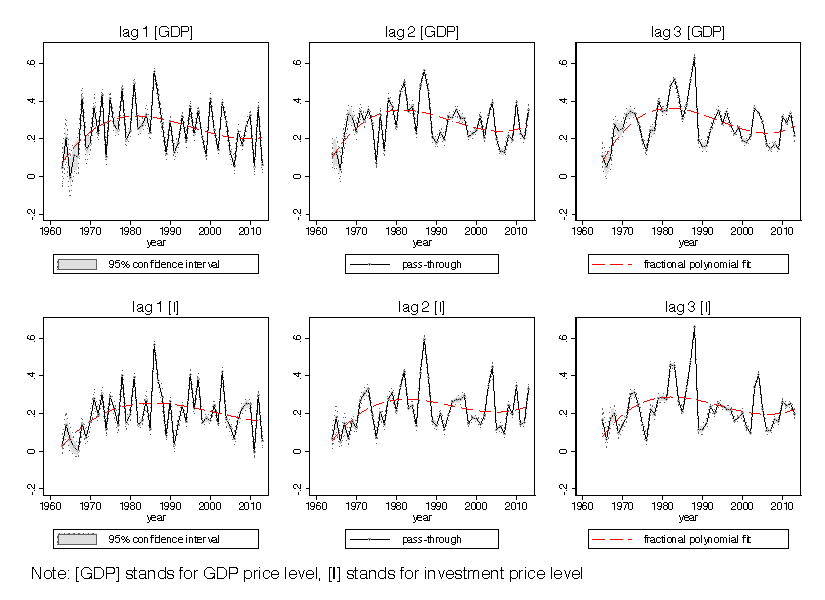
\includegraphics[width=1\textwidth]{firststage.pdf}
\label{fig:firststage}
\end{figure}

The predicted unit values in $t$, $\hat{p}_{k,ij,t}$ are constructed by augmenting the unit values observed in $t-l$ with the change in the common cost component, given the estimate of the pass-through $\hat{\alpha}^\nu_{t-l}$:
\begin{eqnarray}
\hat{p}_{k,ij,t}&=&{p}_{k,ij,t-l}\left(\frac{P^\nu_{i,t}}{P^\nu_{i,t-l}}\right)^{\hat{\alpha^\nu_{t,l}}}\label{eqn:uvpred}
\end{eqnarray}

As the past unit values are a very strong predictor of current unit values, we are not worried about the strength of our instrument, notwithstanding the fact that economy-wide cost shocks explain a relatively small fraction of variation in landed sectoral prices.
%\footnote{The adjustment of past unit values for the common cost component weakly increases the correlation between past and current unit values.} 
%Still, this may worry us as to the weakness of our instrument.
%Recall however that the instrument is actually the adjusted past unit value.
%Past unit values have a very strong correlation with present unit values.
%The correlation between adjusted past unit values and current unit values is slightly higher.

We estimate (\ref{eqn:nlestimation}) while replacing current unit values with the predicted unit values $\hat{p}_{k,ij,t-l}$ from (\ref{eqn:uvpred}). To keep as many years as possible, we opt for the smallest time lag ($l=1$). Figure \ref{fig:instr} presents the results.
\footnote{Reported confidence intervals do not take into account the fact that we are using predicted unit values $\hat{p}_{k,ij,t-l}$  on the right-hand side of the equation: we do not know how to make the adjustment in that setting}
%The choice of the lag is associated with a trade-off.
%The shorter the lag, the more data we can use.
%However, if demand shocks in the destination are persistent, the covariance between the lagged price and the demand shock in the error term may remain positive if the first lag is used.

\begin{figure}[H]
\caption{Estimated $1-\sigma$, predicted unit values}
\includegraphics[width=1\textwidth]{"1ere regression 3e partie_instrumented".pdf}
\label{fig:instr}
\end{figure}

The absolute value of the estimated trade elasticity $|1-\sigma|$ has increased by 60\% from 1963 to 2013. The predicted trade elasticity equals $-.65$ in 2013. 
This corresponds to an annual increase of .9\% per year.\footnote{The estimated annualized growth rate is significant at the 1\% level, the 95\% confidence interval is between 0.7\% and 1.2\% (not taking into account though the uncertainty around yearly estimates).} The evolution of the parameter is much more pronounced when predicted unit values are used in the estimation, suggesting that price endogeneity may indeed be affecting not only the level but also the evolution of the estimated elasticity.

\if 0
As a falsification test, we verify that variations of the unit price are not explained by past or future variations of domestic costs.
We thus estimate the following equation:

\[\ln {{p}_{k,ij,t}}-\ln {{p}_{k,ij,t-l}}={{\alpha }_{k,t}}\ln \left( \frac{P_{i,t}^{v}}{P_{i,t-l}^{v}} \right)+{{\beta }_{k,t}}\ln \left( \frac{P_{i,t+2}^{v}}{P_{i,t+1}^{v}} \right)+\gamma \ln \left( \frac{P_{i,t-3}^{v}}{P_{i,t-4}^{v}} \right)+{{\varepsilon }_{k,ij,t,l}}\] 
\fi

%Instrumenting: motivation and results (old)
%previous procedure used GDP price index to predict evolution of own price relatively to evolution of price in the destination (as a function of price evolution of each partner, weighted by respective market shares).
%For each destination market, we compute the mean evolution of GDP price levels in current US dollars of its trading partners, weighted by their market shares in this destination.
%This amounts to computing the evolution of the relevant real exchange rate for each specific bilateral trade relation.
%Third, we compute a hypothetical relative price at time \textit{t} for each exporter in each market as the product of its relative price at time (\textit{t}${-}$1) and the evolution of its GDP price level between \textit{t} and (\textit{t}-1) relatively to all other trading partners in this destination.
%Fourth, we predict the relative price of each exporter in each destination at time \textit{t} by regressing its observed relative price on this hypothetical relative price.
%This gives an instrumented relative price for each exporter which depends only on its past relative price and the relative evolution of its GDP price level.
%Finally, we estimate equation {\hyperref[ref-002]{ }} using these instrumented relative prices instead of the observed relative prices.

%What is the economic significance of a reduction in the degree of structural heterogeneity? The reduction in the number of zeros in the bilateral sectoral trade matrix illustrates that over the last five decades a growing number of countries started producing an increasingly similar set of goods.
%In the Armington framework the composite good each country exports is horizontally differentiated.
%If consumer perception of the degree of differentiation across places of production is decreasing in the similarity of the product mix that countries supply to world markets, then an increasing Armington trade elasticity, i.e. an increasing sensitivity of consumers to price differences of country-specific product bundles, would indicate an increasing similarity of country-specific composite goods.
%Our focus on product heterogeneity is motivated by several considerations.
%Firstly, the Armington framework provides a straightforward aggregation procedure which allows focusing on the substitutability of country-composite goods rather than on sector-specific heterogeneity in the level and evolution of the elasticity of substitution pointed out by previous studies.
%Second, the economic significance of our results may be rather general.
%In particular, increasing similarity of product mix implies decreasing cross-sectoral heterogeneity in ability, i.e. reduction in Ricardian-type heterogeneity.
%This paper is the first to provide empirical evidence on the reduction in the degree of structural heterogeneity of the economy in the last five decades by means of estimating annual trade elasticities.
%If zeros are a statistical feature and given that sectoral Armington elasticities are finite, reduction in nb of zeros means that domestic price of the good has decreased enough for the volume of trade to increase sufficiently in order to be recorded in trade statistics.
%Hence, dispersion in prices of domestically produced goods decreases overtime.
%In Ricardian framework this is equivalent to reduction in dispersion of technological ability, e.g.
%a reduction in the strength of comparative advantage or an increase in the Ricardian trade elasticity.
%Evidence of this is provided in Levchenko and Zhang.
%As documented in L\&Z, strong heterogeneity across countries: in certain countries no reduction in dispersion.
%This could explain muted evolution of aggregate trade elasticity in our sample (additional robustness check would consist in verifying that increase in trade elasticity is magnified in the superbalanced sample and/or for the fixed set of goods).
%In the framework of the many-good many-country Ricardian model an increasing trade elasticity would be observed if the process of technological upgrading proceeded at a quicker pace in sectors lagging furthest behind the world technology frontier.
%Specifically, if trade integration facilitated international technology diffusion and allowed quicker technological upgrading in initially least productive sectors, it could result in reduced intersectoral dispersion in country-specific technology stocks.
%This evolution would lead to an increase in the sensitivity of trade flows to trade costs.
%Levchenko2016 find that countries' technological capabilities have become more homogeneous across sectors over 1950-2010, reducing the strength of comparative advantage in determining trade flows.

%0 We provide a robustness check by estimating the evolution of the heterogeneity parameter for aggregate bilateral trade on a different dataset.
%We use the BACI dataset which reports bilateral trade data at the HS-1992 6-digit disaggregation level for 1995-2009.
%The accuracy of the relative prices of country-composite goods constructed with this dataset is improved because the harmonization procedure applied by Gaulier2010 in constructing BACI yields much better-quality unit values while substantially reducing the number of observations with lacking unit value.
%As a result, at the 6-digit level, less than 7\% of total reported trade in BACI has missing unit values.
%This is reduced to 1-3\% of total trade when the data is aggregated to the 4-digit level, as opposed to more than 10\% in the raw COMTRADE data we originally used.
%Another advantage is that the share of ztf in BACI is stable in 1995-2009 as opposed to relatively strong fluctuations in the share of ztf overtime in our original dataset.
%The disadvantage of BACI is that it covers only a relatively short period compared to the years over which the distance puzzle exists.
%Obviously, we do not expect to reproduce exactly the results obtained with our original dataset because the trade classification and its level of aggregation are different.
%the increase in the elasticity is much steeper on the BACI dataset.
%This finding supports the idea that our benchmark estimation likely provides a lower bound on the increase in the aggregate trade elasticity.

\subsection{ Is there a distance puzzle left?}

This section has provided empirical evidence on the evolution of the aggregate substitutability parameter for world trade from 1963 to 2013.
In the Armington framework, this substitutability parameter $(1-\sigma)$ corresponds to the aggregate trade elasticity  $\epsilon$.
We find that this parameter has increased by 22\% between 1963 and 2009 in the baseline estimation, and by 60\% when prices are instrumented.
Section 1 has shown that the distance elasticity of trade ($\delta$)has increased by 4\% over the same period in the baseline estimate.
A naïve combination of these two results suggests, there is no distance puzzle left in the framework of the Armington model in as much as the elasticity of trade costs to distance ($\rho$) has decreased by 15\% in 1963-2013.
More formally, we run Monte Carlo estimation of the mean and standard deviation of $\rho$ defined as $\frac{\delta}{1-\sigma}$. Figure \ref{fig:rho} gives the results for the baseline estimation, the instrumented estimation and the superbalanced sample.
Years where the estimated standard deviation is too large or the estimation of $\sigma$ did not converge are dropped out. The resulting precision of the measure of $\rho$ is not what we would like.
That is partially because of the use of the Huber-White method to correct standard errors in the gravity equation.
Still, in all cases, the point estimates suggest a decrease of $\rho$ by 13\% in the baseline estimate, 27\% using the instrumented method and 23\% in the superbalanced sample.
%\footnote{The elasticity decreases by 5\% when the evolution of $\rho$ is computed from the ratio of trends, and by 7\% when it is computed as the trend of the ratios.}
Increasing perceived substitutability of country-specific composite goods contributes to the non-decreasing distance elasticity of trade.


\begin{figure}[H]
	\caption{Estimated $\rho$ }
	\includegraphics[width=1\textwidth]{"graph_rho".pdf}
	\label{fig:rho}
\end{figure}

%The reduction in the elasticity of trade costs to distance is even more pronounced if we focus on 1970-2009.
%As shown by (Hummels 2007), this period is characterized by a new phenomenon: the fact that air transportation starts playing a substantial role in world trade.
%The instrumented Armington elasticity increases by 19\% in this period while the evolution of the distance elasticity is best described as flat.
%It follows that the elasticity of trade costs to distance has decreased by at least 17\% in 1970-2009.


What is the economic interpretation of an increasing substitutability parameter measured on aggregate data? 

First, the degree of perceived similarity of country-composite goods may have increased.
Since the 1960s, a growing number of countries started producing a set of goods similar to that of developed countries.
This process has increased the number of available varieties and, potentially, their degree of similarity.\footnote{(Schott 2004) documents increased similarity in the set of exported goods of US trade partners while (\cite{Broda2006}) document the increase in the number of imported varieties since the 1970s.
} 

Second, composition effects may have lead to changes in the parameter estimated on aggregate data.
If the reduction in trade barriers has led to the expansion in the range of traded goods, trade in previously non-traded sectors could modify measured substitutability of country-composite goods.
Non-uniform reductions in sectoral trade costs would also modify the composition of world trade, leading to a change in the substitutability parameter measured on aggregate data.
However, at first approximation, the rising importance of manufactures compared to primary products in world trade should have reduced substituability.

Ideally, we would like to separate out the impact of composition and sector-specific effects to quantify the net effect of increased perceived similarity of country-composite goods.
This is however impossible because, as shown by (Imbs et M\'{e}jean 2013), the parameter estimated on aggregate data cannot be mimicked by a weighted average of sectoral parameters.
The bottom line is that an increase in measured substitutability for country-composite goods is consistent with complex competition dynamics in price and quality documented by (Amiti et Khandelwal 2013) as well as with increased vertical specialization of countries within sectors documented by (Fontagn\'{e}, Gaulier, et Zignago 2008).

%maybe here introduce discussion of alternative frameworks (whether result is relevant if move away from Armington); discuss restrictiveness of assumptions in EK-ChaneyMelitz (or) threshold effect
\section{Conclusion}

The estimated effect of distance in gravity equations has not decreased in the past fifty years despite substantial innovation in transportation and communication that should have reduced the relative effect of distance: this is the `distance puzzle'.
Using COMTRADE 4-digit bilateral trade data in 1962-2013, this paper finds that the evolution of the elasticity of trade flows to trade costs, referred to as the `trade elasticity', provides a direct explanation of the increasing distance elasticity of trade.
Increased sensitivity of trade flows to relative prices has more than compensated the reduction in the elasticity of trade costs to distance.

The paper proceeds in three steps.
First, it shows that the distance puzzle is a feature of our data by estimating yearly cross-section gravity equations.
In the baseline estimation the distance coefficient has increased by 4\% from 1962 to 2013.
This result holds when we correct for changes in the sample of trading partners and the composition of world trade.
%Taking into account FTAs seems to solve the distance puzzle, but this might be an artefact of their growing importance: introducing FTAs dummies amounts to adding a time-growing number of proximity controls in the estimation.

Second, the paper suggests a method to measure structural heterogeneity in the Armington framework.
In the main theoretical foundations of the gravity equation the distance coefficient is the product of the elasticity of trade costs to distance and a measure of heterogeneity.
In the Armington framework, heterogeneity is inter-country and intra-sector.
The trade elasticity corresponds to the degree of perceived substitutability of country-specific varieties of each good, which can be approximated by studying the relations between the prices and the market share of importers in destination markets.

Third, the paper estimates the evolution of the trade elasticity in the Armington framework, i.e. the substitution elasticity between country composite goods.
It uses 4-digit unit values as proxies for sectoral prices.
%In our method, unobserved unit values for zero trade flows lead to an overestimation bias that is reduced over time.
%As the estimated elasticity still increases in absolute value this%Guillaume DaudinGD2016-04-20T14:47:00Z Guillaume DaudinGD Guillaume DaudinGD Guillaume Daudin Guillaume Daudin GD GD 2016-04-20T14:47:00Z 2016-04-20T14:47:00Z 0 while the overestimation bias is reduced, 0 while the overestimation bias is reduced,
% evolution provides a lower bound on the increase in the absolute value of the underlying trade elasticity.
Depending on the method of estimation, the estimated elasticity increases by between 22\% and 60\% between 1963 and 2013.

Combining the estimation of the distance coefficient and the elasticity of trade to trade costs, we can then compute the elasticity of trade costs to distance. Alas, that estimate is bound to be very measured with uncertainty, because it the the ratio of two uncertain results. Still, the point estimates are our best guess at the estimated values and are compatible with a decrease of the elasticity of trade costs to distance of between 13\% and 23\% between 1963 and 2013.
%This reduction in the elasticity of trade costs to distance is even more pronounced if we focus on the period in which air transportation starts playing an important role in bilateral trade.
%We find that from 1970 to 2009 the elasticity of trade costs to distance has decreased by 17\% while the perceived substitutability of countries' product bundles has increased by at least 19\%.



%these lines should be at point where biblio should appear
%\bibliographystyle{harvard} %alternative bibliography styles
%\bibliographystyle{acm}
\bibliographystyle{chicago}
%\bibliographystyle{aer}
\bibliography{Armington_biblio_inbibtex}
%\end{spacing}

\clearpage
\appendix
\revLA{I updated numbers in the text and graphs by defining the superbalanced sample for 1962-2013.}
\section{Full and superbalanced samples} \label{app:E}
The full sample contains 205 reporters (R) and 227 partners (P) listed in tables \ref{tab:list1} and \ref{tab:list2} below.
`S' indicates that the country is present in the superbalanced sample.


In the full sample, several countries shift from reporting trade on an individual basis to reporting trade jointly with another country.
This is the case of Belgium and Luxembourg, as well as Eritrea and Ethiopia.
For consistency, we use a single country identifier for each of these two pairs.
A single country identifier is also used for Yougoslavia and for Serbia and Montenegro.
Figure \ref{fig:pairpresence} shows the distribution of pairs in the full sample according to the number of years in which the pair reports a positive amount of trade.

%graph updated for 1962-2013
\begin{figure}[h!]
\begin{center}
\setlength{\fboxrule}{1pt} %makes border lines thick
\setlength{\fboxsep}{.1in} %increases distance to border
\fbox{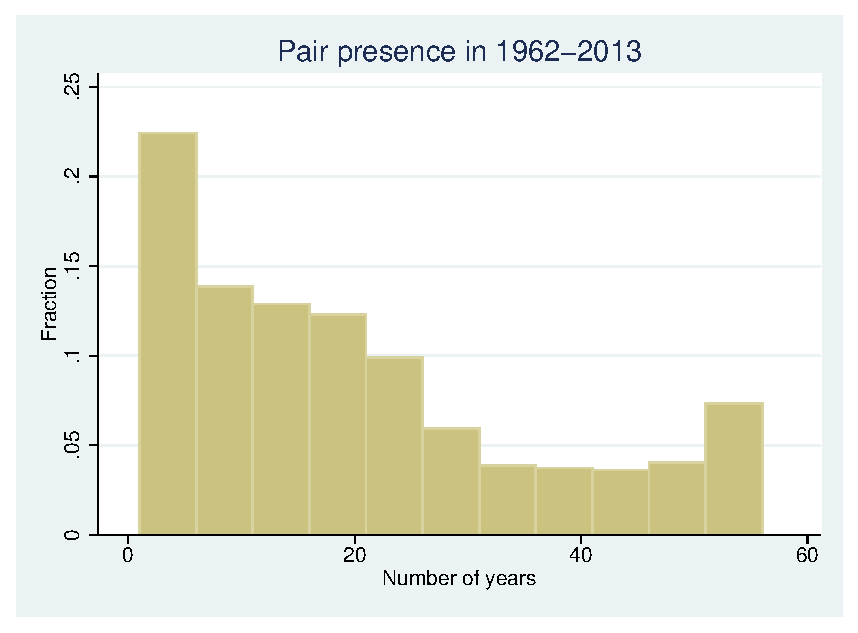
\includegraphics[trim = 0.5mm 0.5mm 0.5mm 8mm, clip, height=2.5in]{nb_years_pair_presence_1962_13.eps}}
\end{center}
\caption{Number of years each pair is present in the sample \label{fig:pairpresence}}
\end{figure}

The superbalanced sample corresponds to the subsample of pairs which trade both ways in each and every year in 1962-2013.
To avoid discarding pairs which fall out of the superbalanced sample because countries split up or reunite at some point in 1962-2013, we introduce several additional single country identifiers before constructing the superbalanced sample.
Consequently, Germany is present in the superbalanced sample.\footnote{A single identifier is used for East, West, and reunited Germany.
A single identifier is used for the Czech Republic, Slovakia, and Czechoslovakia.
A single identifier is used for the USSR and the 15 countries formed after the USSR split up.
The 15 countries which constituted the USSR are absent from the superbalanced sample because the USSR is never a reporter to COMTRADE.
The Czech Republic and Slovakia also drop out because there is no other country in the sample with which they have two-way trade in every year.} 
%it is strange that Czech and Slovak Republics drop out from superbalanced sample...do not trade both ways with reunited Germany..maybe because DDR does not report trade in all years to COMTRADE.

The superbalanced sample comprises 786 trading pairs and corresponds to 32 countries.
This is less than the 992 pairs which would be observed if each reporter traded both ways with every other country.
Indeed, the set of countries which trade with every other country in each year and which we refer to as the `square sample' comprises just 21 countries (420 pairs).
Trade coverage in the superbalanced sample decreases from 68 to 39\% of total trade over 1962-2013 while it is reduced from 54 to 28\% for the square sample (see Figure \ref{fig:coverage}).


%graph updated for 1962-2013
\begin{figure}[h]
\begin{center}
\setlength{\fboxrule}{1pt} %makes border lines thick
\setlength{\fboxsep}{.1in} %increases distance to border
\fbox{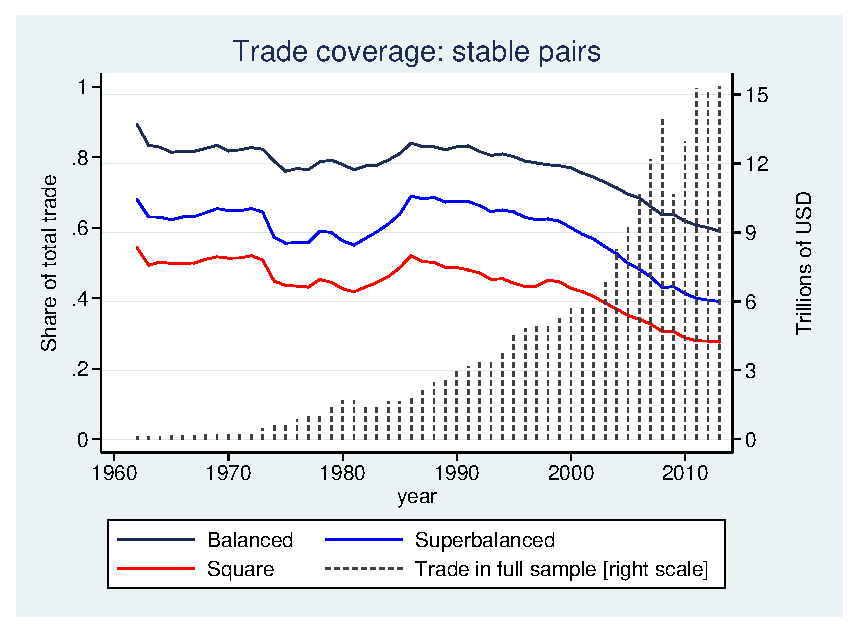
\includegraphics[trim = 0.5mm 0.5mm 0.5mm 8.5mm, clip, height=2.5in]{trade_coverage_1962.eps}}
\end{center}
\caption{Trade coverage in 1962-2013 \label{fig:coverage}}
\end{figure}
%graph updated for 1965-2013
\begin{figure}[h!]
\begin{center}
\setlength{\fboxrule}{1pt} %makes border lines thick
\setlength{\fboxsep}{.1in} %increases distance to border
\fbox{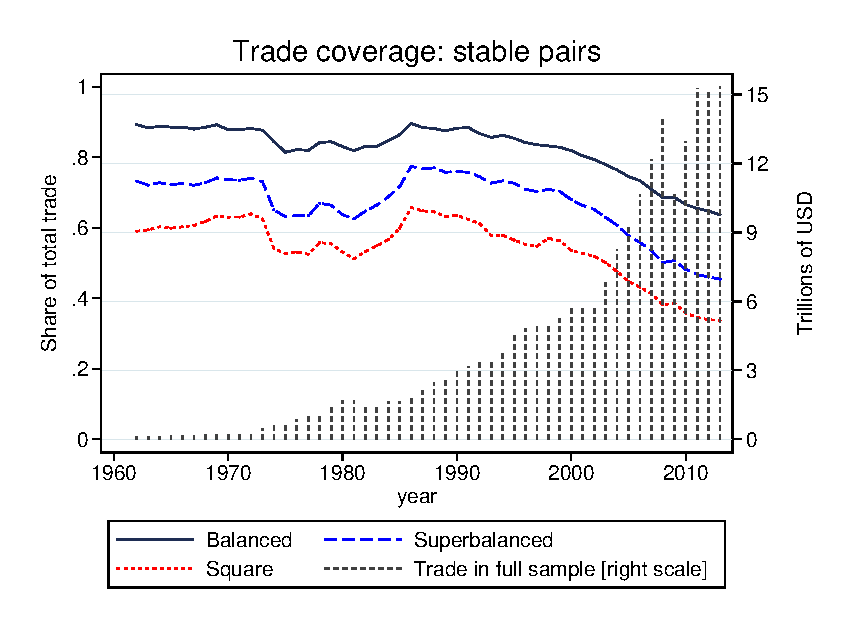
\includegraphics[trim = 0.5mm 0.5mm 0.5mm 8.5mm, clip, height=2.5in]{trade_coverage_1965.eps}}
\end{center}
\caption{Trade coverage in 1965-2013 \label{fig:superbal6513}}
\end{figure}

To check the sensitivity of trade coverage to the choice of the benchmark year we redefine the set of stable pairs as partners trading both ways in each year in 1965-2013.\footnote{The number of reporters increases from 70 in 1962 to 86 in 1965 to 111 in 1970 and 129 in 1975.
But the reduction in trade coverage between the 1970s and the 1990s is qualitatively similar if we choose 1970 or 1975.} The superbalanced sample for 1965-2013 contains 1286 pairs that comprise 42 countries (out of 1722 possible pairs).
The square sample for 1965-2013 contains 23 countries (506 pairs).

As illustrated in Figure \ref{fig:superbal6513}, the evolution of trade coverage is not sensitive to the choice of the starting year.
Albeit from a higher level (73\% in 1965), trade coverage drops to 45\% by 2013.
Indeed, the main reason for the reduction in trade coverage since the mid-1990s is due to the absence of China and of Central and Eastern European countries from the superbalanced sample.
These countries drop out because they do not report trade to COMTRADE until the more recent period.\footnote{For example, China reports trade to UN COMTRADE in 1987-2013.} 

Another way to check the sensitivity of trade coverage to the choice of the starting year is to compute the evolution of trade coverage for the sample of pairs which trade both ways in a specific year.
The difference with the superbalanced sample is that we now relax the constraint that the pair have two-way trade in every year in 1962-2013.
The share of total annual trade attributable to two-way pairs in 1962 and in 1965 is shown in Figure \ref{fig:reciprocal}.
As previously, the level but not the evolution of trade coverage is affected by the choice of the starting year.

%graph updated for 1962(1965)-2013
\begin{figure}[h!]
\begin{center}
\setlength{\fboxrule}{1pt} %makes border lines thick
\setlength{\fboxsep}{.1in} %increases distance to border
\fbox{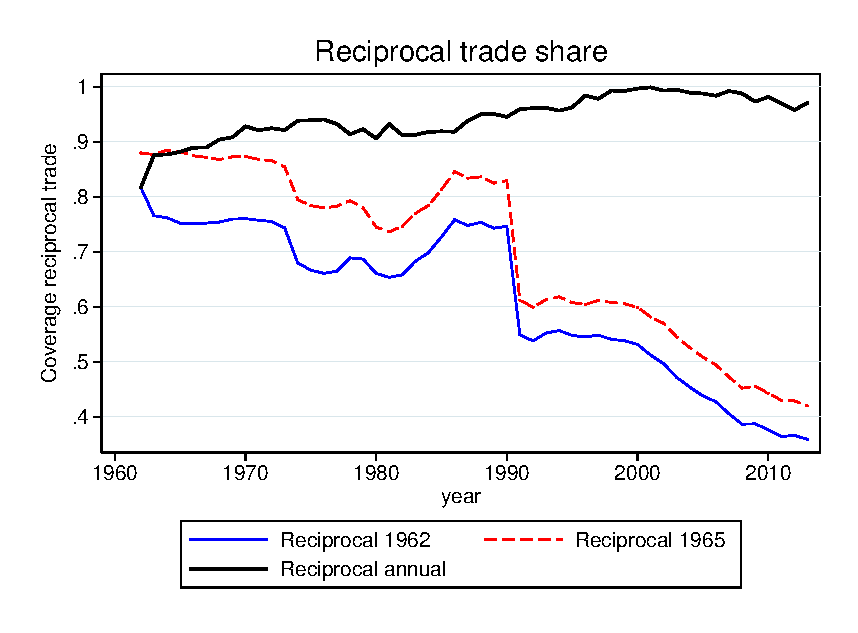
\includegraphics[trim = 0.5mm 0.5mm 0.5mm 8.5mm, clip, height=2.5in]{recip_coverage_62_65.eps}}
\end{center}
\caption{Trade coverage in reciprocal trade \label{fig:reciprocal}}
\end{figure}

\cite{Helpman2008} document that the enlargement of the set of trading partners did not contribute in a major way to the growth of world trade in 1970-1997 because most of the increase was driven by pairs which traded both ways in 1970.
We nuance this finding by showing that since the mid-1990s new reciprocal trade relationships did contribute strongly to the growth of world trade.
Figure \ref{fig:reciprocal} illustrates that while more than 70\% (resp.
80\%) of world trade in 1990 is attributable to pairs that traded both ways in 1962 (resp.
1965), less than 40\% (resp.
50\%) is still attributable to such pairs in 2013.
  

We document that these new trade relationships were formed between countries trading both ways.
To illustrate, Figure \ref{fig:reciprocal} also shows the share of total trade attributable to pairs which trade both ways in a given year (in black).
Since the 1990s more than 95\% of total annual trade takes place between pairs which trade both ways.
One-way trade flows represent a marginal and decreasing share of world trade.
The greater frequency of one-way trade relationships observed in the early years of the sample may be in part attributable to the fact that the number of countries reporting trade to COMTRADE was initially relatively small.
Consequently, reported zeros may be at least in part statistical zeros, i.e.
non-zero trade flows reported as zeros due to missing reports to COMTRADE.


%list of countries updated for 1962-2013 (minor breaches of alphabetic order b/c naming conventions change between latest and previous samples)
\begin{table}
\caption {List of countries in the full and superbalanced samples \label{tab:list1}} 
\begin{tabular}{|l|c|l|c|l|c|}
\hline
{\bf Country name} & {\bf Status} & {\bf Country name} & {\bf Status} & {\bf Country name} & {\bf Status } \\
\hline
Afghanistan &  {\it R;P} & French Polynesia &  {\it R;P} & N.
Mariana Islands &          P \\

   Albania &  {\it R;P} & French S.
Antartic terr.
&          P &     Norway &  {\it R;P} \\

   Algeria &  {\it R;P} &      Gabon &  {\it R;P} &       Oman &  {\it R;P} \\

   Andorra &  {\it R;P} &     Gambia &  {\it R;P} &   Pakistan &  {\it R;P} \\

    Angola &  {\it R;P} &    Georgia &  {\it R;P} &      Palau &          P \\

  Anguilla &  {\it R;P} &   \bf Germany &  {\bf R;P;S} &     Panama (Fm Panama Cz) &  {\it R;P} \\

Antigua-Barbuda &  {\it R;P} &     Ghana &  {\it R;P} & Papua New Guinea &  {\it R;P} \\

 \bf Argentina &  {\bf R;P;S} &  Gibraltar &          P &  \bf Paraguay &  {\bf R;P;S} \\

   Armenia &  {\it R;P} &  \bf Greece &  {\bf R;P;S} &       Peru &  {\it R;P} \\

     Aruba &  {\it R;P} &  Greenland &  {\it R;P} & \bf Philippines &  {\bf R;P;S} \\

 Australia &  { R;P} &    Grenada &  {\it R;P} &   Pitcairn &          P \\

   Austria &  { R;P} & Guadeloupe &  {\it R;P} &     Poland &  {\it R;P} \\

Azerbaijan &  {\it R;P} &  Guatemala &  {\it R;P} &  \bf Portugal &  {\bf R;P;S} \\

   Bahamas &  {\it R;P} &     Guinea &  {\it R;P} &      Qatar &  {\it R;P} \\

   Bahrain &  {\it R;P} & Guinea-Bissau &  {\it R;P} &    Reunion &  {\it R;P} \\

Bangladesh &  {\it R;P} &     Guyana &  {\it R;P} &    Romania &  {\it R;P} \\

  Barbados &  {\it R;P} &      Haiti &  {\it R;P} & Russian Federation &  {\it R;P} \\

   Belarus &  {\it R;P} &   Honduras &  {\it R;P} &     Rwanda &  {\it R;P} \\

  \bf Belgium-Luxembourg &  {\bf R;P;S} & \bf Hong Kong &  {\bf R;P;S} & St.
Helena &          P \\

    Belize &  {\it R;P} &    Hungary &  {\it R;P} & St.
Kitts and Nevis &  {\it R;P} \\

     Benin &  {\it R;P} &  \bf Iceland &  {\bf R;P;S} &  St.
Lucia &  {\it R;P} \\

   Bermuda &  {\it R;P} &      India &  {\it R;P} & St.
Vincent-Grenadines &  {\it R;P} \\

    Bhutan &  {\it R;P} &  Indonesia &  {\it R;P} &      Samoa &  {\it R;P} \\

   Bolivia &  {\it R;P} &       Iran &  {\it R;P} & San Marino &          P \\

Bosnia-Herzeg.
&  {\it R;P} &       Iraq &  {\it R;P} & Sao Tome-Principe &  {\it R;P} \\

  Botswana &  {\it R;P} &   Ireland &  {R;P} & Saudi Arabia &  {\it R;P} \\

  \bf Brazil &  {\bf R;P;S} &  \bf Israel &  {\bf R;P;S} &    Senegal &  {\it R;P} \\

Br.
Virgin Islands &          P &   \bf Italy &  {\bf R;P;S} & Serbia-Montenegro &  {\it R;P} \\

Brunei Darussalam &  {\it R;P} &    Jamaica &  {\it R;P} & Seychelles &  {\it R;P} \\

  Bulgaria &  {\it R;P} &   \bf Japan &  {\bf R;P;S} & Sierra Leone &  {\it R;P} \\
  
Burkina Faso &  {\it R;P} &     Jordan &  {\it R;P} & \bf Singapore &  {\bf R;P;S} \\

 Burma (Myanmar)   & {\it R;P}  &  Kazakstan &  {\it R;P} &   Slovakia &  {\it R;P} \\

   Burundi &  {\it R;P} &      Kenya &  {\it R;P} &   Slovenia &  {\it R;P} \\
  
  Cambodia &  {\it R;P} &   Kiribati &  {\it R;P} & Solomon Islands &  {\it R;P} \\

  Cameroon &  {\it R;P} &   \bf Korea &  {\bf R;P;S} &    Somalia &  {\it R;P} \\

  \bf Canada &  {\bf R;P;S} & DPR of Korea &          P & South Africa &  {\it R;P} \\
\hline
\end{tabular}    
\end{table}

\begin{table}
\caption {List of countries in the full and superbalanced samples: Contd.
\label{tab:list2}} 
\begin{tabular}{|l|c|l|c|l|c|}
\hline
{\bf Country name} & {\bf Status} & {\bf Country name} & {\bf Status} & {\bf Country name} & {\bf Status } \\
\hline
Cape Verde &  {\it R;P} &     Kuwait &  {\it R;P} & Soviet Union &          P \\

Cayman Islands &          P & Kyrgyzstan &  {\it R;P} &   \bf  Spain &  {\bf R;P;S} \\

C.African Republic &  {\it R;P} &    Lao PDR &  {\it R;P} &  Sri Lanka &  {\it R;P} \\

 Chad &  {\it R;P} &     Latvia &  {\it R;P} & St.
Pierre and Miquelon &  {\it R;P} \\

   \bf Chile &  {\bf R;P;S} &    Lebanon &  {\it R;P} &      Sudan &  {\it R;P} \\
   
 China &  {\it R;P} &    Lesotho &  {\it R;P} &   Suriname &  {\it R;P} \\

Christmas Island &          P &    Liberia &  {\it R;P} &  Swaziland &  {\it R;P} \\

Cocos Islands &          P &      Libya &  {\it R;P} &   \bf Sweden &  {\bf R;P;S} \\

 \bf Colombia &  {\bf R;P;S} &  Lithuania &  {\it R;P} & \bf Switzerland &  {\bf R;P;S} \\

   Comoros &  {\it R;P} & Luxembourg &  {R;P} &      Syria &  {\it R;P} \\

   Congo &  {\it R;P} & Macau (Aomen) &  {\it R;P} &      &  \\

Dem.
Rep.
of Congo &  {\it R;P} & Macedonia  &  {\it R;P} & Tajikistan &  {\it R;P} \\

Cook Islands &  {\it R;P} & Madagascar &  {\it R;P} &   Tanzania &  {\it R;P} \\

Costa Rica &  {\it R;P} &     Malawi &  {\it R;P} &  \bf Thailand &  {\bf R;P;S} \\

   Croatia &  {\it R;P} &  \bf Malaysia &  {\bf R;P;S} &       Togo &  {\it R;P} \\

      Cuba &  {\it R;P} &   Maldives &  {\it R;P} &    Tokelau &          P \\

    Cyprus &  {\it R;P} &       Mali &  {\it R;P} &      Tonga &  {\it R;P} \\

Czech Republic &  {\it R;P} &      Malta &  {\it R;P} & Trinidad-Tobago &  {\it R;P} \\

Czechoslovakia &  {\it R;P} & Marshall Islands &          P &  \bf Tunisia &  {\bf R;P;S} \\

C\^ote d'Ivoire &  {\it R;P} & Martinique &  {\it R;P} &   \bf Turkey &  {\bf R;P;S} \\

  \bf Denmark &  {\bf R;P;S} & Mauritania &  {\it R;P} & Turkmenistan &  {\it R;P} \\

  Djibouti &  {\it R;P} &  Mauritius &  {\it R;P} & Turks-Caicos Islands &  {\it R;P} \\

  Dominica &  {\it R;P} &   \bf Mexico &  {\bf R;P;S} &     Tuvalu &  {\it R;P} \\

Dominican Republic &  {\it R;P} & Micronesia  &          P &     Uganda &  {\it R;P} \\

East Germany (DDR) &  {R;P} &    Moldova &  {\it R;P} &    Ukraine &  {\it R;P} \\

East Timor &  {\it R;P} &   Mongolia &  {\it R;P} & United Arab Emirates &  {\it R;P} \\

   Ecuador &  {\it R;P} & Montserrat &  {\it R;P} & \bf United Kingdom &  {\bf R;P;S} \\

     Egypt &  {\it R;P} &    Morocco &  {\it R;P} &     \bf  USA &  {\bf R;P;S} \\

El Salvador &  { R;P} & Mozambique &  {\it R;P} &    Uruguay &  {\it R;P} \\

Equatorial Guinea &          P &    Namibia &  {\it R;P} & Uzbekistan &          P \\

   Eritrea &  {\it R;P} &      Nauru &          P &    Vanuatu &  {\it R;P} \\

   Estonia &  {\it R;P} &      Nepal &  {\it R;P} & \bf Venezuela &  {\bf R;P;S} \\

  Ethiopia &  {\it R;P} & Netherland Antilles &  {\it R;P} &  Vietnam (Fm Vietnam Rp) &  {\it R;P} \\

Falkland Islands &          P & \bf Netherlands &  {\bf R;P;S} & Wallis-Futuna &  {\it R;P} \\

 Palestine & {\it R;P}  & New Caledonia &  {\it R;P} & West Germany (FRG) &  {R;P} \\

      Fiji &  {\it R;P} & New Zealand &  {\it R;P} & Western Sahara &          P \\

   Finland &  {R;P} &  Nicaragua &  {\it R;P} &      Yemen &  {\it R;P} \\

\bf  France &  {\bf R;P;S} &      Niger &  {\it R;P} & Yugoslavia (Serbia-Mont.) &  {\it R;P} \\

French Guiana & {\it R;P}  &  Nigeria &  {\it R;P} &     Zambia &  {\it R;P} \\

Niue & P & Norfolk Island  & P &   Zimbabwe &  {\it R;P} \\
\hline
\end{tabular}    
\end{table}


\end{document}

